\chapter{残余应力和变形}

残余应力和变形计算是多尺度问题,小尺度采用热循环计算,如图\ref{fig:4.0.0.3}左列,大尺度采用固有应变法,如图\ref{fig:4.0.0.3}右列。在热循环计算中采用生死单元法,生死单元有两种情况,一种是计算区域是有真实的变化,需要添加网格单元,暂时称为激活单元,如图\ref{fig:4.0.0.1},另外一种情况是计算区域没有变化,通过改变材料系数增加单元,暂时称为静单元,我们采用激活单元和静单元的混合形式,逐层增加网格,然后再对每一层修改材料系数,如图\ref{fig:4.0.0.2}。计算和图\ref{fig:4.0.0.4}中研究问题类似,具体几何参数可以调整。具体问题可以先计算热传导,再计算热弹塑性,热弹塑性采用最简单的理想塑性本构。

\begin{figure}[!htbp]
  \centering
  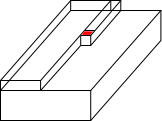
\includegraphics[height=3cm]{fig/4/1.png}
  \caption{激活单元}
  \label{fig:4.0.0.1}
\end{figure}

\begin{figure}[!htbp]
  \centering
  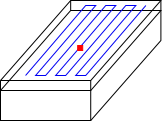
\includegraphics[height=3cm]{fig/4/2.png}
  \caption{激活单元和静单元混合形式}
  \label{fig:4.0.0.2}
\end{figure}

\begin{figure}[!htbp]
  \centering
  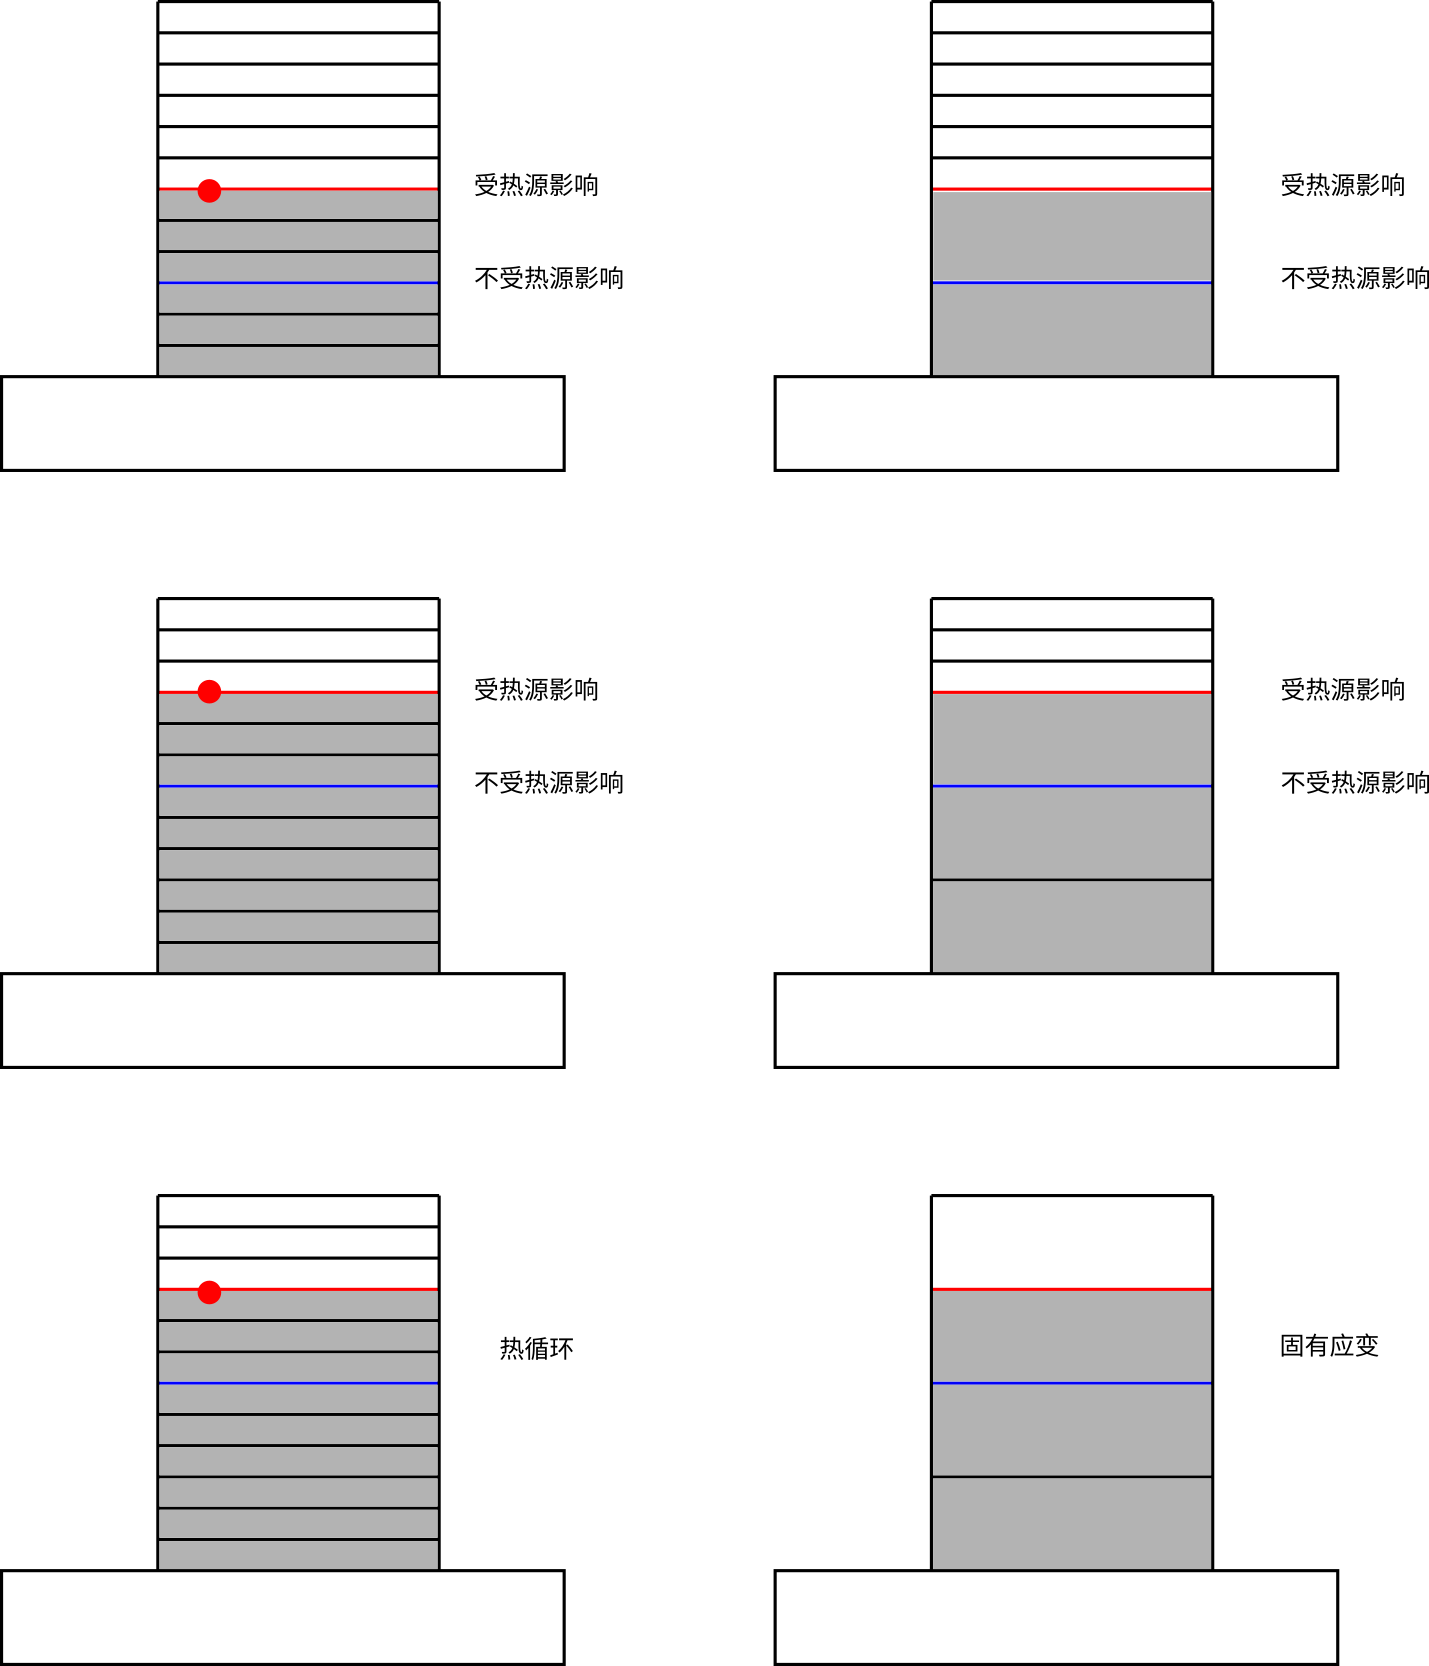
\includegraphics[height=9cm]{fig/4/3.png}
  \caption{热循环和固有应变法}
  \label{fig:4.0.0.3}
\end{figure}

\begin{figure}[!htbp]
  \centering
  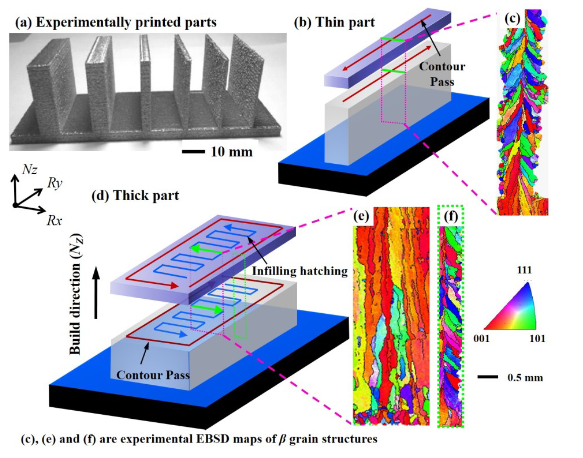
\includegraphics[height=7cm]{fig/4/4.png}
  \caption{材料相场到固有应变法}
  \label{fig:4.0.0.4}
\end{figure}

\section{小尺度热循环生死单元法}
\subsection{泊松方程}

偏微分方程定义为
\begin{align}\label{eq:4.1.1:1}
  -\Delta u = f \qquad \mathrm{in}\ \Omega\,.
\end{align}

Dirichlet和Neumann边界条件定义为
\begin{subequations}
  \begin{align}\label{eq:4.1.1:2}
    u &= g_{\mathrm D} &\mathrm{on}\ \Gamma_{\mathrm D}\,, \\
    \partial_{\mathbf n}u & = g_{\mathrm N} &\mathrm{on}\ \Gamma_{\mathrm N}\,.
  \end{align}
\end{subequations}

散度定理(Divergence Theorem)为

\begin{align*}
  \int_{\Omega}\nabla \cdot \mathbf w \ud x = \int_{\Gamma}\mathbf n \cdot \mathbf w \ud s\,.
\end{align*}

格林公式(Green's Formula)为

\begin{align*}
  \int_{\Omega}\mathbf w \cdot \nabla v  \ud x  + \int_{\Omega}\nabla\cdot\mathbf w  v  \ud x = \int_{\Gamma}\mathbf n \cdot \mathbf w v\ud s \,.
\end{align*}

如果$\mathbf w=\nabla u$得到

\begin{align}\label{eq:4.1.1:5}
  \int_{\Omega}\nabla u \cdot \nabla v  \ud x  + \int_{\Omega}\nabla\cdot\nabla u  v  \ud x = \int_{\Gamma}\mathbf n \cdot \nabla u v\ud s \,.
\end{align}

方程\eqref{eq:4.1.1:1}两边乘以$v$并做积分得到

\begin{align}\label{eq:4.1.1:6}
  -\int_{\Omega}\Delta uv\ud x &= \int_{\Omega}fv\ud x\,.
\end{align}

将\eqref{eq:4.1.1:5}带入\eqref{eq:4.1.1:6}得到
   
\begin{align}\label{eq:4.1.1:7}
  \int_{\Omega}\nabla u \cdot \nabla v  \ud x = \int_{\Omega}fv\ud x + \int_{\Gamma}\mathbf n \cdot \nabla u v\ud s\,.
\end{align}

根据\eqref{eq:4.1.1:7}定义变分形式。找到$u\in H^1_g$满足

\begin{align}   
  a(u,v)=(f,v) \qquad \forall v\in H^1_0\,.
\end{align}

找到$u_h\in S_{h,g}$满足

\begin{align}   
  a(u_h,\chi)=(f,\chi) \qquad \forall \chi\in S_{h,0}\,.
\end{align}

\begin{align}   
  Ax = b
\end{align}

已知条件如下:
\begin{subequations}
  \begin{align*}
   &u=\mathrm e^{x_1+x_2}\,,\\
   &\Omega:=(0,1)^2\,,\\
   &\Gamma_{\mathrm D}:=\{x|x_1=0\}\bigcup\{x|x_2=0\}\,,\\
   &\Gamma_{\mathrm N}:=\Gamma\setminus\Gamma_{\mathrm D}\,, \\
   &g_{\mathrm D}=\mathrm e^{x_1+x_2}\,,\\
   &g_{\mathrm N}=\mathrm e^{x_1+x_2}\,,\\
    &f=-2\mathrm e^{x_1+x_2}\,.
  \end{align*}
\end{subequations}

表\ref{tab:4.1.1:1}是收敛速度验证,图\ref{fig:4.1.1:1}是level 8的结果图。
\begin{table}[!htbp]\label{tab:4.1.1:1}
  \centering
  \begin{tabular}{c|r|l|l}
    level      &    dof   &         error  &         roc\\
    \hline
    5         &     2113  &         0.00028354  &    3.990265924 \\
    \hline
    6         &     8321  &         7.0922e-05  &    3.9979132 \\
    \hline
    7         &     33025 &         1.7732e-05  &    3.999661629 \\
    \hline
    8         &     131585 &        4.4333e-06  &    3.999729321
  \end{tabular}
  \caption{the Poisson equation, mixed b.c., 2D}
\end{table}

\begin{figure}[!htbp]
  \centering
  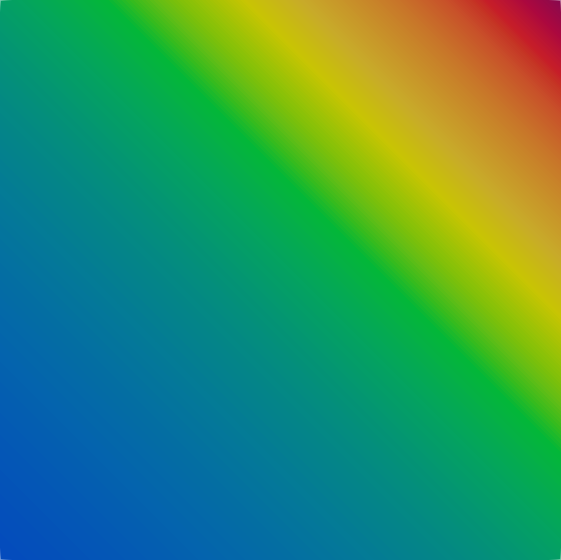
\includegraphics[height=3cm]{fig/4/fig:1.1.1:1.png}
  \caption{the Poisson equation, mixed b.c., 2D}
  \label{fig:4.1.1:1}
\end{figure}

已知条件如下:

\begin{subequations}
  \begin{align*}
   &u=\mathrm e^{x_1+x_2+x_3}\,,\\
   &\Omega:=(0,1)^3\,,\\
   &\Gamma_{\mathrm D}:=\{x|x_1=0\}\bigcup\{x|x_2=0\}\bigcup\{x|x_3=0\}\,,\\
   &\Gamma_{\mathrm N}:=\Gamma\setminus\Gamma_{\mathrm D}\,, \\
   &g_{\mathrm D}=\mathrm e^{x_1+x_2+x_3}\,,\\
   &g_{\mathrm N}=\mathrm e^{x_1+x_2+x_3}\,,\\
    &f=-3\mathrm e^{x_1+x_2+x_3}\,.
  \end{align*}
\end{subequations}


   
表\ref{tab:4.1.1:2}是收敛速度验证,\ref{fig:4.1.1:2}是level 6的结果图。

\begin{table}[!htbp]\label{tab:4.1.1:2}
  \centering
  \begin{tabular}{c|r|l|l}
    level    &      dof   &         error  &         roc \\
    \hline
    3      &        2465  &         0.010258    &    3.776857087 \\
    \hline
    4      &        17985 &         0.0026009  &     3.944019378 \\
    \hline
    5      &        137345   &      0.00065152  &    3.992049361 \\
    \hline
   6      &        1073409   &     0.00016299  &    3.997300448
  \end{tabular}
  \caption{the Poisson equation, mixed b.c., 3D}
\end{table}

\begin{figure}[!htbp]
  \centering
  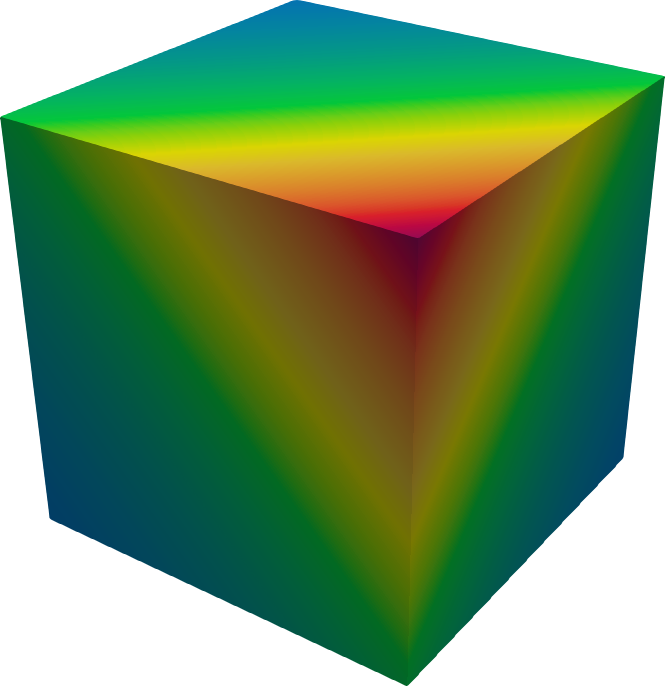
\includegraphics[height=3cm]{fig/4/fig:1.1.1:2.png}
  \caption{the Poisson equation, mixed b.c., 3D}
  \label{fig:4.1.1:2}
\end{figure}


\subsection{热传导方程}

偏微分方程定义为

\begin{align}
  u_t - \Delta u = f \qquad \mathrm{in}\ \Omega\times\mathrm R_+\,.
\end{align}

Dirichlet和Neumann边界条件定义为
\begin{subequations}	   
  \begin{align}	   
    u &= g_{\mathrm D} &\mathrm{on}\ \Gamma_{\mathrm D}\times\mathrm R_+\,,\\
    \partial_{\mathbf n}u & = g_{\mathrm N} &\mathrm{on}\ \Gamma_{\mathrm N}\times\mathrm R_+\,.
  \end{align}
\end{subequations}	   

初始条件定义为
\begin{align}		   
  u(\cdot,0) = v \qquad \mathrm{in}\ \Omega\,.
\end{align}

找到$u\in H^1_g$满足
\begin{align}		   
  (u_t,\varphi) + a(u,\varphi)=(f,\varphi) \qquad \forall \varphi\in H^1_0, t>0\,.
\end{align}

找到$u_h\in S_{h,g}$满足
\begin{align}		   
  (u_{h,t},\chi) + a(u_h,\chi)=(f,\chi) \qquad \forall \chi\in S_{h,0}, t>0\,.
\end{align}

对时间进行离散
\begin{align}
   \overline\partial_t U^n = \frac{U^n - U^{n-1}}{k}\,.
\end{align}

找到$U^n\in S_{h,g}$满足
\begin{align}
  \left(\frac{U^n - U^{n-1}}{k},\chi\right) + a(U^n,\chi)=(f^n,\chi) \qquad \forall \chi\in S_{h,0}
\end{align}

\begin{align}
  \left(U^n,\chi\right) + ka(U^n,\chi)=(kf^n,\chi) + \left(U^{n-1},\chi\right)
\end{align}

\begin{align}
  Ax = b
\end{align}

已知条件如下:
\begin{subequations}	   
  \begin{align*}	      
   &u=\mathrm e^t \mathrm e^{x_1+x_2}\,,\\
   &\Omega:=(0,1)^2\,,\\
   &\Gamma_{\mathrm D}:=\{x|x_1=0\}\bigcup\{x|x_2=0\}\,,\\
   &\Gamma_{\mathrm N}:=\Gamma\setminus\Gamma_{\mathrm D}\,, \\
   &g_{\mathrm D}=\mathrm e^t \mathrm e^{x_1+x_2}\,,\\
   &g_{\mathrm N}=\mathrm e^t \mathrm e^{x_1+x_2}\,,\\
   &f=-\mathrm e^t \mathrm e^{x_1+x_2}\,,\\
    &v=\mathrm e^{x_1+x_2}\,.
  \end{align*}
\end{subequations}	   

表\ref{tab:4.1.2:1}是收敛速度验证,图\ref{fig:4.1.2:1}是level 8的结果图。

\begin{table}[!htbp]\label{tab:4.1.2:1}
  \centering
  \begin{tabular}{c|r|l|l}
    level     &     dof      &      error  &         roc \\
    \hline
    3,7     &        145     &      0.007936  &      3.891003024 \\
    \hline
    4,9   &         545       &    0.0019999 &      3.96819841 \\
    \hline
    5,11  &         2113   &       0.00050099  &    3.991896046 \\
    \hline
    6,13  &         8321  &        0.0001253   &    3.998324022 
  \end{tabular}
  \caption{the Heat equation, mixed b.c., 2D, $T=0.5$}
\end{table}

\begin{figure}[!htbp]
  \centering
  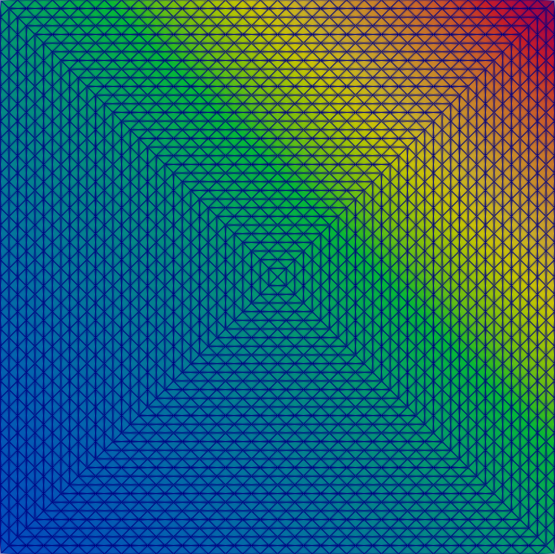
\includegraphics[height=3cm]{fig/4/fig:1.1.2:1.png}
  \caption{the Heat equation, mixed b.c., 2D, $T=0.5$}
  \label{fig:4.1.2:1}
\end{figure}


已知条件如下:

\begin{subequations}	   
  \begin{align*}	      
   &u=\mathrm e^t\mathrm e^{x_1+x_2+x_3}\,,\\
   &\Omega:=(0,1)^3\,,\\
   &\Gamma_{\mathrm D}:=\{x|x_1=0\}\bigcup\{x|x_2=0\}\bigcup\{x|x_3=0\}\,,\\
   &\Gamma_{\mathrm N}:=\Gamma\setminus\Gamma_{\mathrm D}\,, \\
   &g_{\mathrm D}=\mathrm e^t\mathrm e^{x_1+x_2+x_3}\,,\\
   &g_{\mathrm N}=\mathrm e^t\mathrm e^{x_1+x_2+x_3}\,,\\
   &f=-2\mathrm e^t\mathrm e^{x_1+x_2+x_3}\,,\\
    &v=\mathrm e^{x_1+x_2+x_3}\,.
  \end{align*}
\end{subequations}	   

表\ref{tab:4.1.2:2}是收敛速度验证,图\ref{fig:4.1.2:2}是level 6的结果图。

\begin{table}[!htbp]\label{tab:4.1.2:2}
  \centering
  \begin{tabular}{c|r|l|l}
    level   &       dof  &          error    &       roc \\
    \hline
    2,5     &    369     &       0.062935 &\\
    \hline
    3,7     &    2465    &       0.016651  &      3.779652874 \\
    \hline
    4,9     &    17985   &       0.0042227  &     3.943211689 \\
    \hline
    5,11    &    137345  &       0.0010577   &    3.992341874
  \end{tabular}
  \caption{the Heat equation, mixed b.c., 3D, $T=0.5$}
\end{table}

\begin{figure}[!htbp]
  \centering
  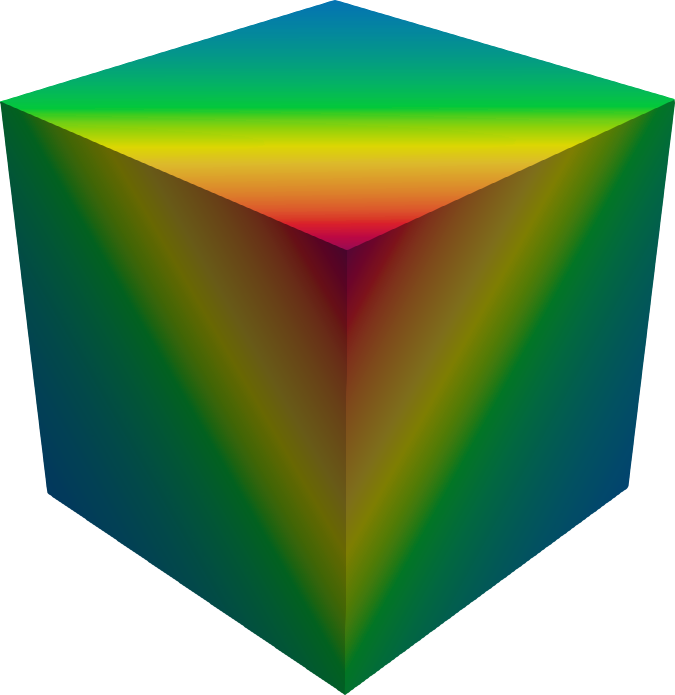
\includegraphics[height=3cm]{fig/4/fig:1.1.2:2.png}
  \caption{   the Heat equation, mixed b.c., 3D, $T=0.5$}
  \label{fig:4.1.2:2}
\end{figure}



\newpage
\subsection{动态显式弹塑}

动态显式弹塑比较了四面体网格和六面体网格的区别,并和Abaqus结果进行了验证。有一个程序inp2geo将Abaqus的inp文件中网格转成.geo格式网格,但是并行有问题。

\begin{figure}[!htbp]
  \centering
  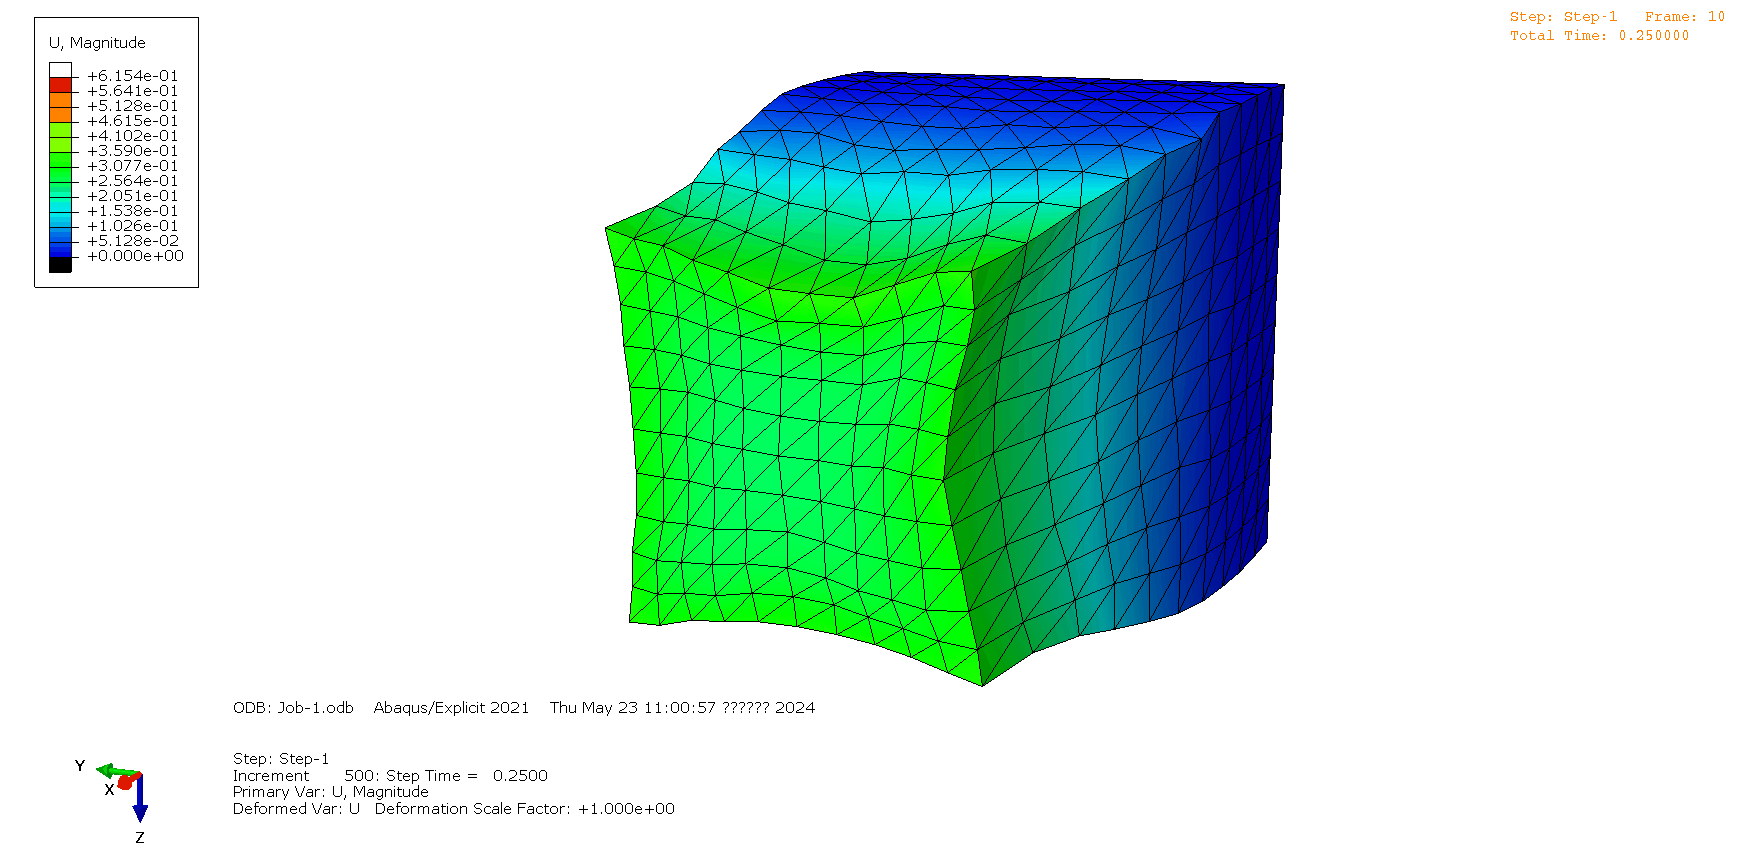
\includegraphics[height=3cm]{fig/4/4.1.5/3.png}
  \caption{动态显式弹塑,弹性模量210,泊松比0.3,塑性屈服0.24,体单元积分点个数为4,边界单元积分点个数为1,时间0.5,结果时间为0.25,总时间步数1000}
  \label{fig:4.1.4:4}
\end{figure}

\begin{figure}[!htbp]
  \centering
  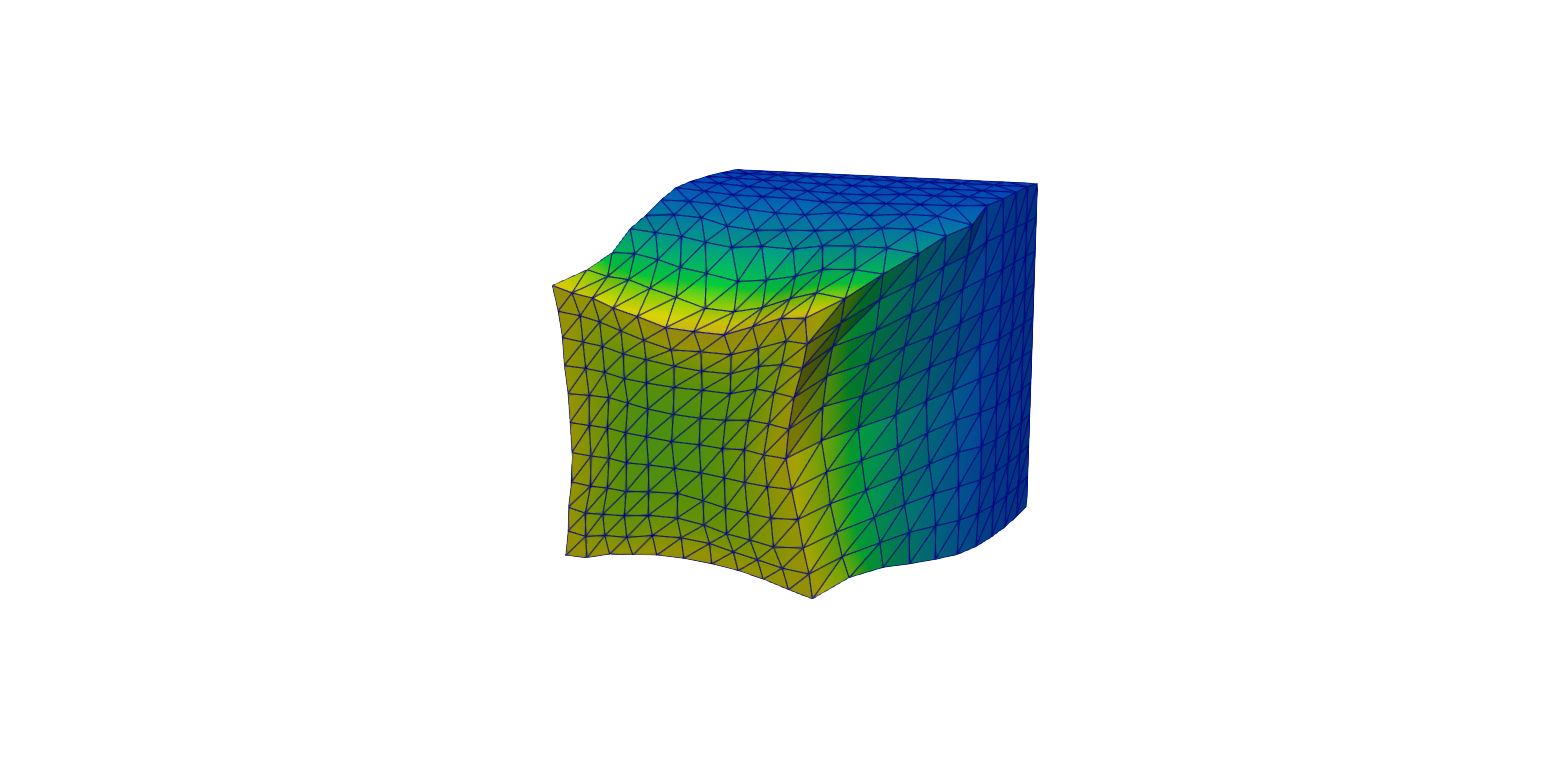
\includegraphics[height=3cm]{fig/4/4.1.5/3-1.png}
  \caption{动态显式弹塑,弹性模量210,泊松比0.3,塑性屈服0.24,体单元积分点个数为4,边界单元积分点个数为1,时间0.5,结果时间为0.25,总时间步数1000}
  \label{fig:4.1.4:4}
\end{figure}

\begin{figure}[!htbp]
  \centering
  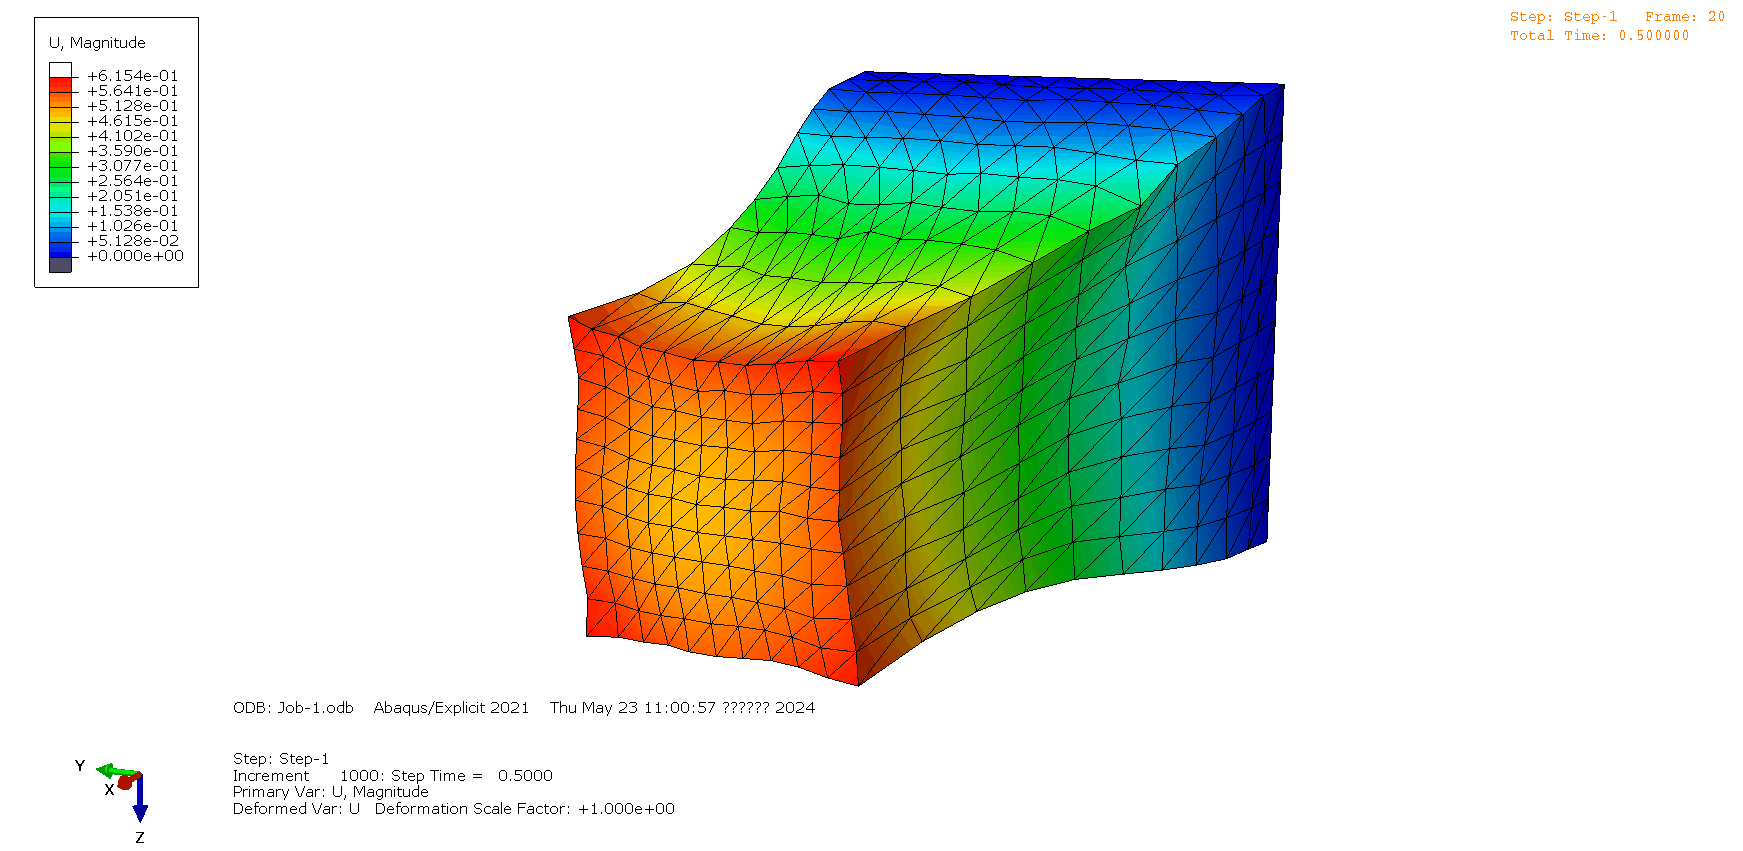
\includegraphics[height=3cm]{fig/4/4.1.5/4.png}
  \caption{动态显式弹塑,弹性模量210,泊松比0.3,塑性屈服0.24,体单元积分点个数为4,边界单元积分点个数为1,时间0.5,结果时间为0.5,总时间步数1000}
  \label{fig:4.1.4:4}
\end{figure}

\begin{figure}[!htbp]
  \centering
  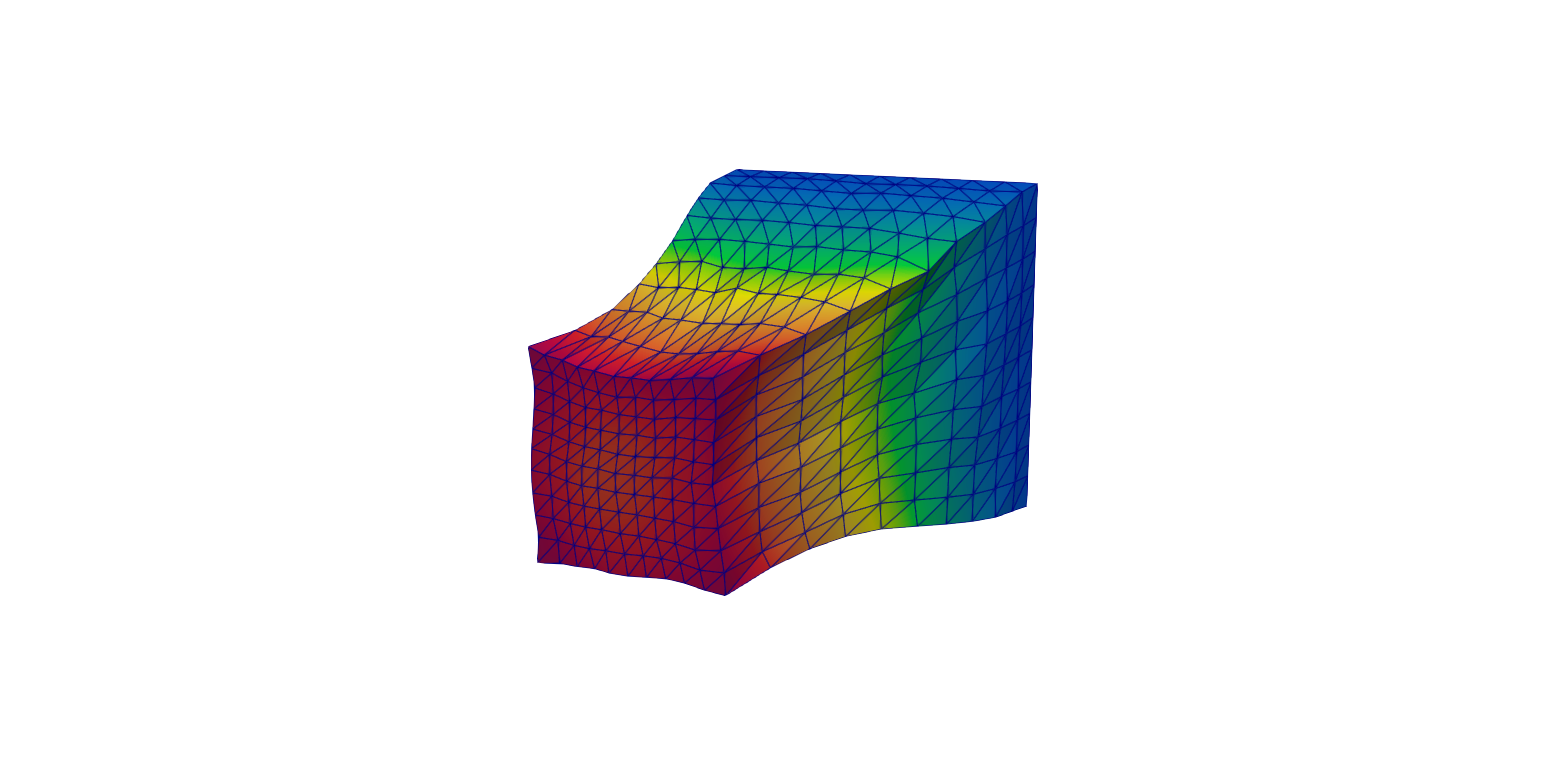
\includegraphics[height=3cm]{fig/4/4.1.5/4-1.png}
  \caption{动态显式弹塑,弹性模量210,泊松比0.3,塑性屈服0.24,体单元积分点个数为4,边界单元积分点个数为1,时间0.5,结果时间为0.5,总时间步数1000}
  \label{fig:4.1.4:4}
\end{figure}

\begin{figure}[!htbp]
  \centering
  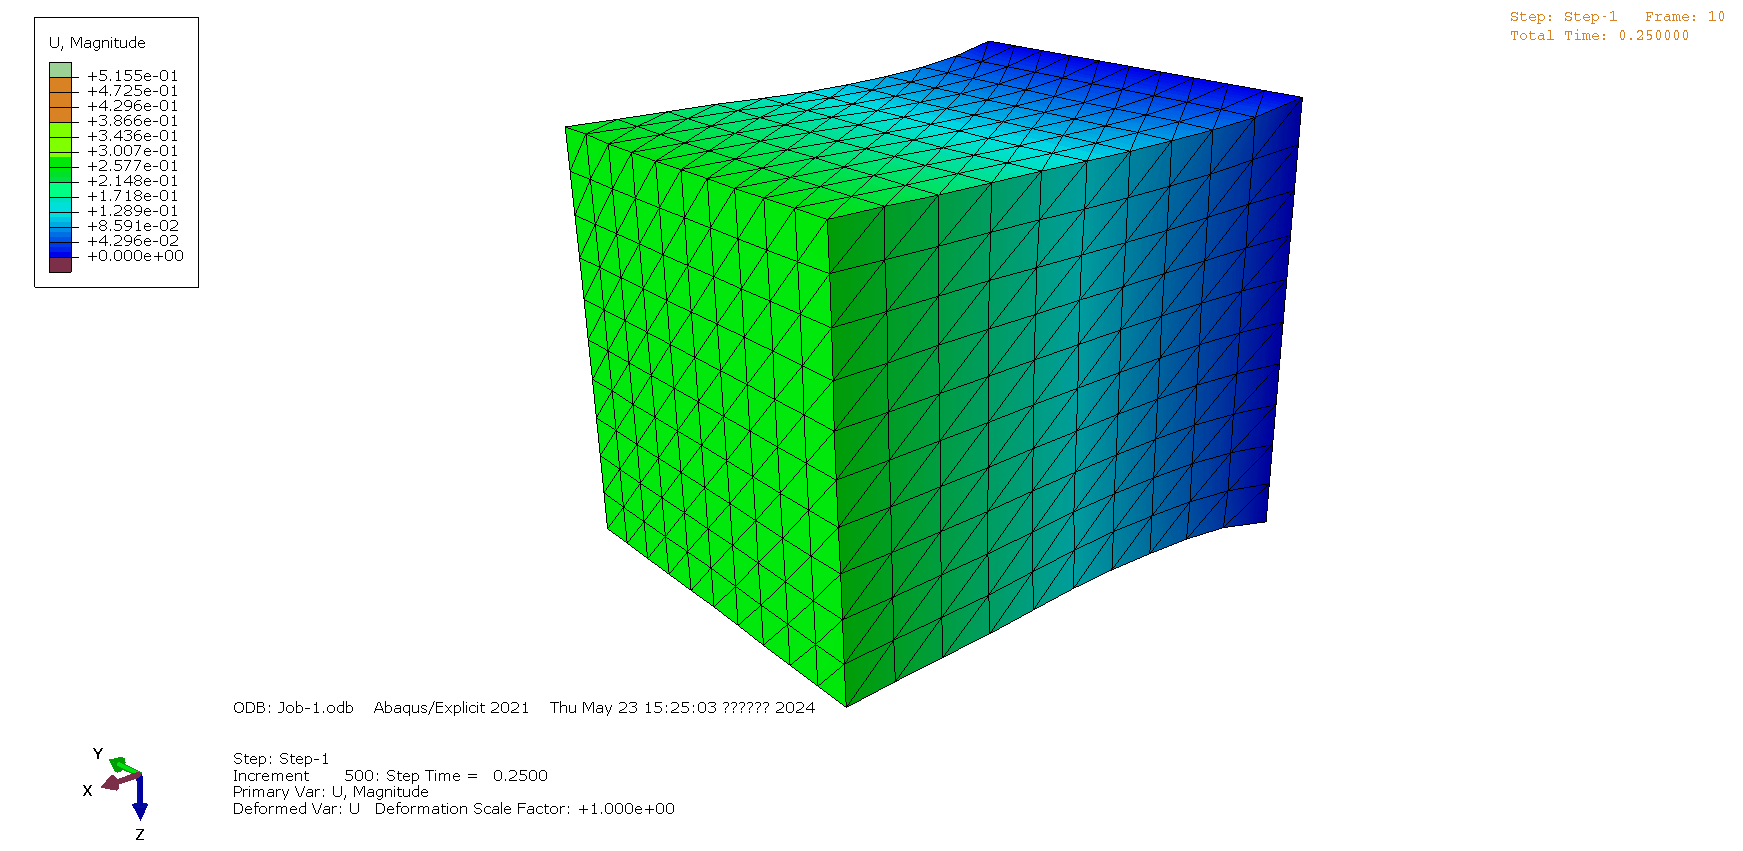
\includegraphics[height=3cm]{fig/4/4.1.5/5.png}
  \caption{动态显式弹塑,弹性模量210,泊松比0.3,塑性屈服1e10,体单元积分点个数为4,边界单元积分点个数为1,时间0.5,结果时间为0.25,总时间步数1000}
  \label{fig:4.1.4:4}
\end{figure}

\begin{figure}[!htbp]
  \centering
  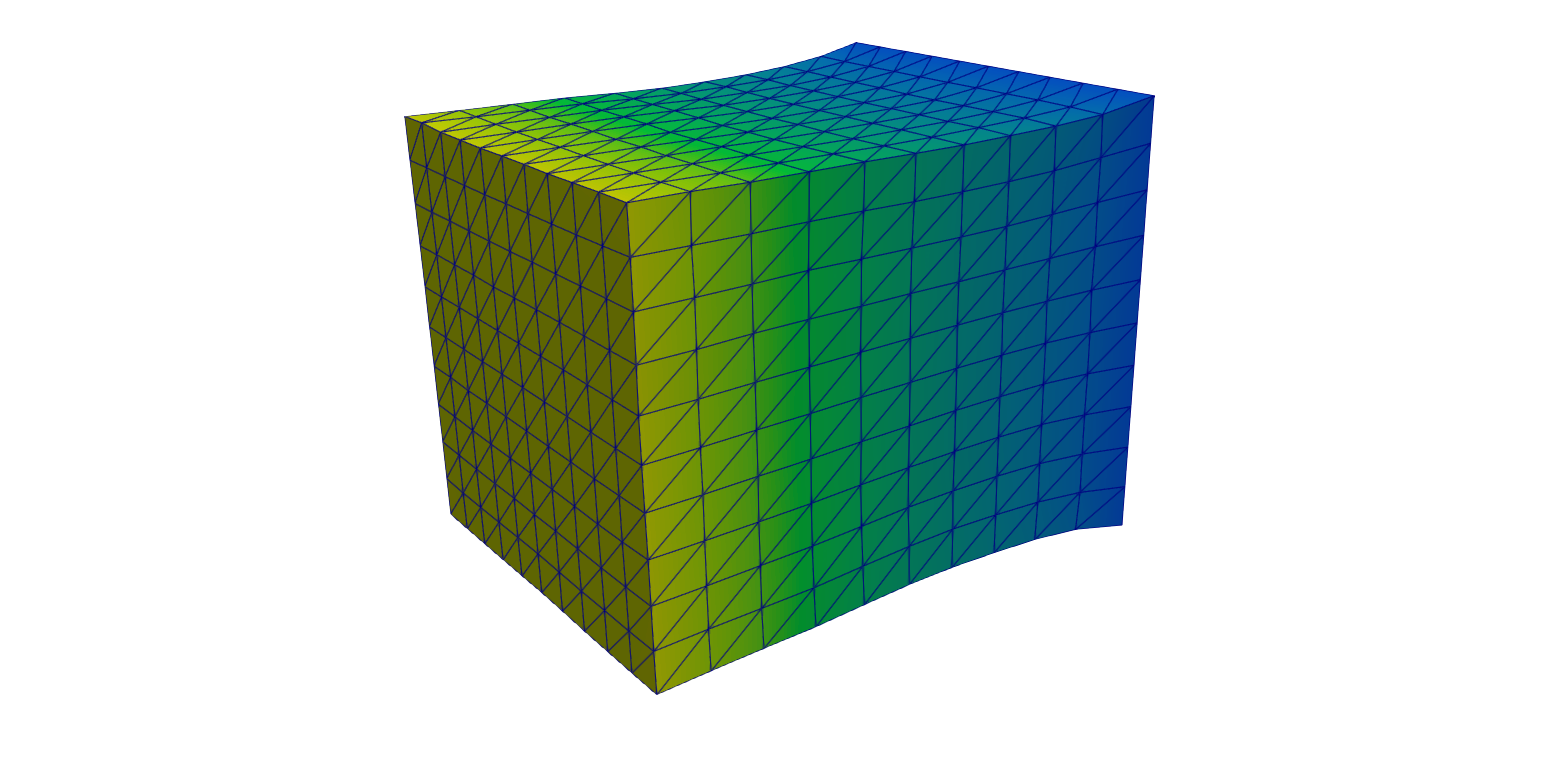
\includegraphics[height=3cm]{fig/4/4.1.5/5-1.png}
  \caption{动态显式弹塑,弹性模量210,泊松比0.3,塑性屈服1e10,体单元积分点个数为4,边界单元积分点个数为1,时间0.5,结果时间为0.25,总时间步数1000}
  \label{fig:4.1.4:4}
\end{figure}

\begin{figure}[!htbp]
  \centering
  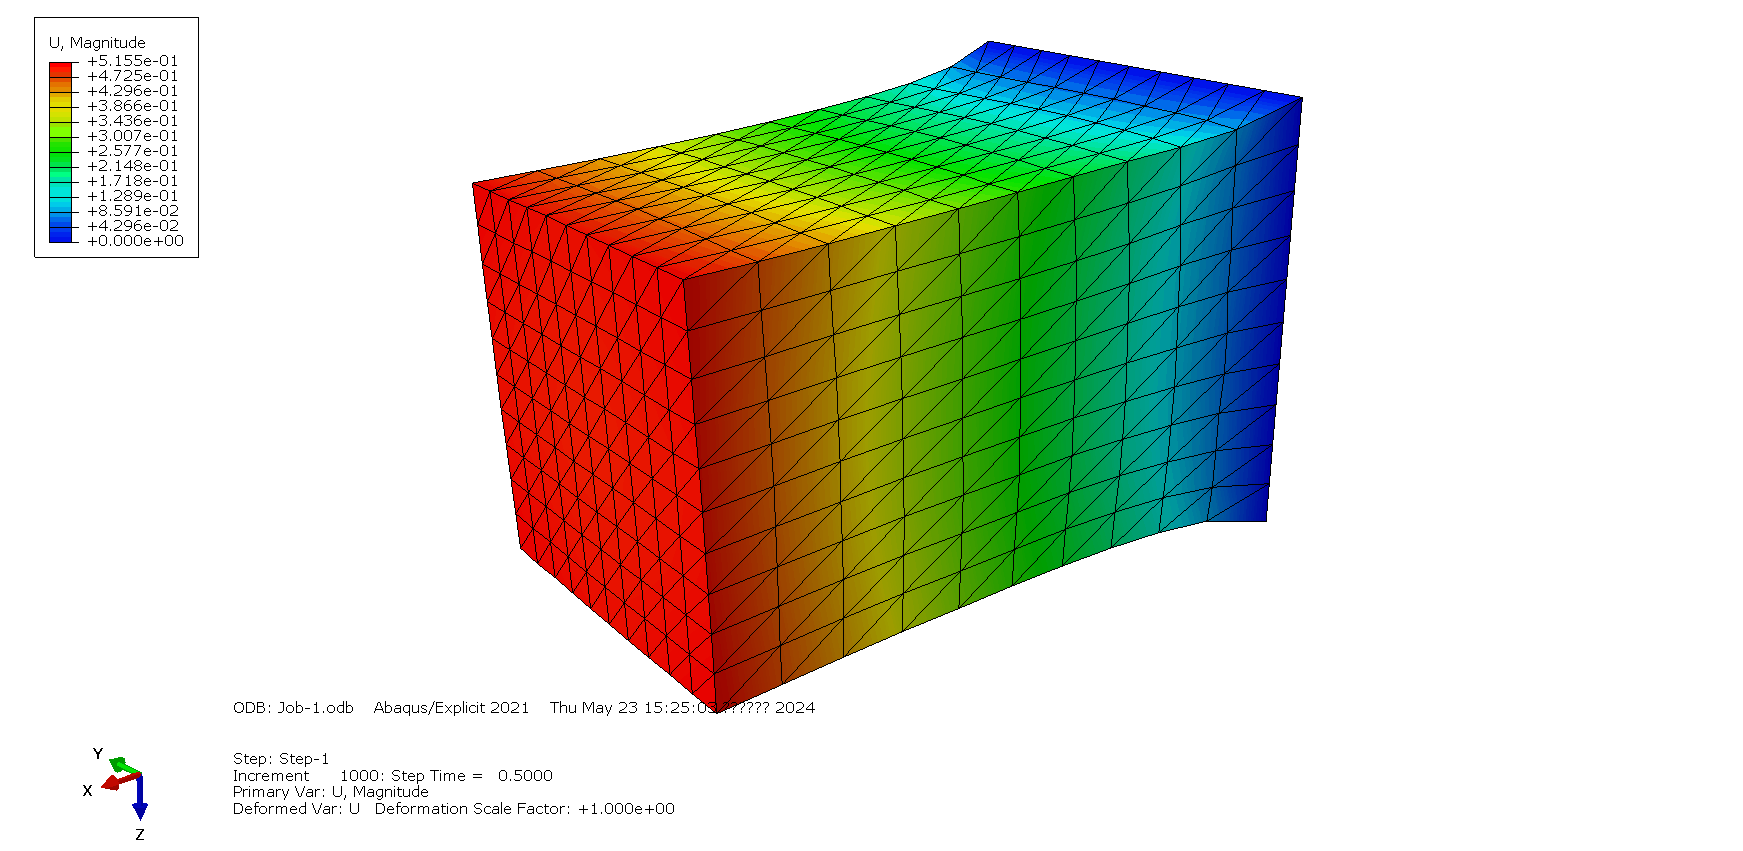
\includegraphics[height=3cm]{fig/4/4.1.5/6.png}
  \caption{动态显式弹塑,弹性模量210,泊松比0.3,塑性屈服1e10,体单元积分点个数为4,边界单元积分点个数为1,时间0.5,结果时间为0.5,总时间步数1000}
  \label{fig:4.1.4:4}
\end{figure}

\begin{figure}[!htbp]
  \centering
  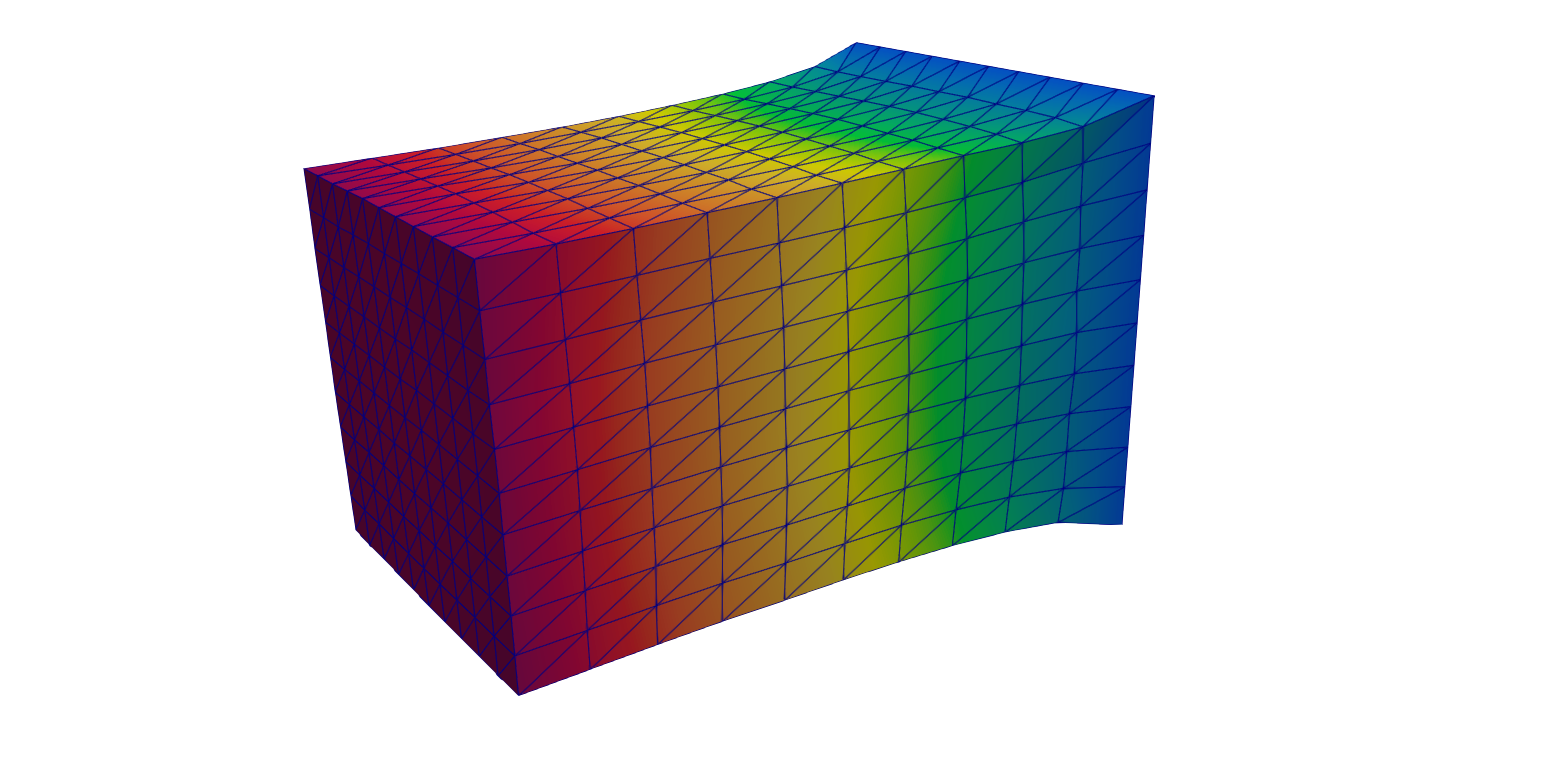
\includegraphics[height=3cm]{fig/4/4.1.5/6-1.png}
  \caption{动态显式弹塑,弹性模量210,泊松比0.3,塑性屈服1e10,体单元积分点个数为4,边界单元积分点个数为1,时间0.5,结果时间为0.5,总时间步数1000}
  \label{fig:4.1.4:4}
\end{figure}

\begin{figure}[!htbp]
  \centering
  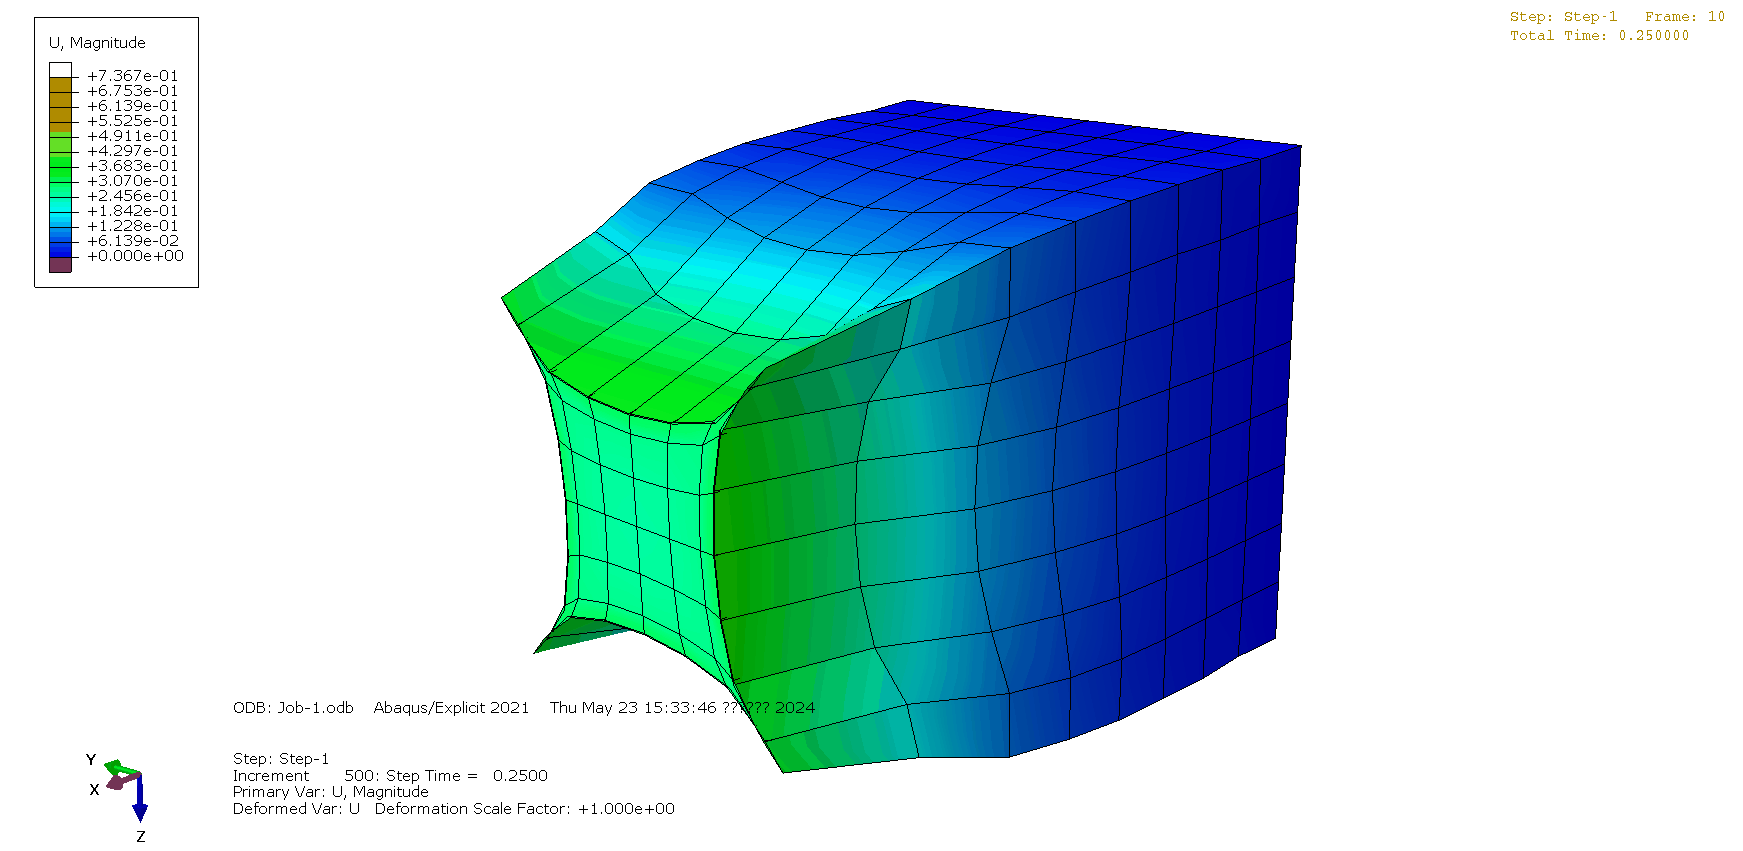
\includegraphics[height=3cm]{fig/4/4.1.5/7.png}
  \caption{动态显式弹塑,弹性模量210,泊松比0.3,塑性屈服0.24,体单元积分点个数为1,边界单元积分点个数为1,时间0.5,结果时间为0.25,总时间步数1000}
  \label{fig:4.1.4:4}
\end{figure}

\begin{figure}[!htbp]
  \centering
  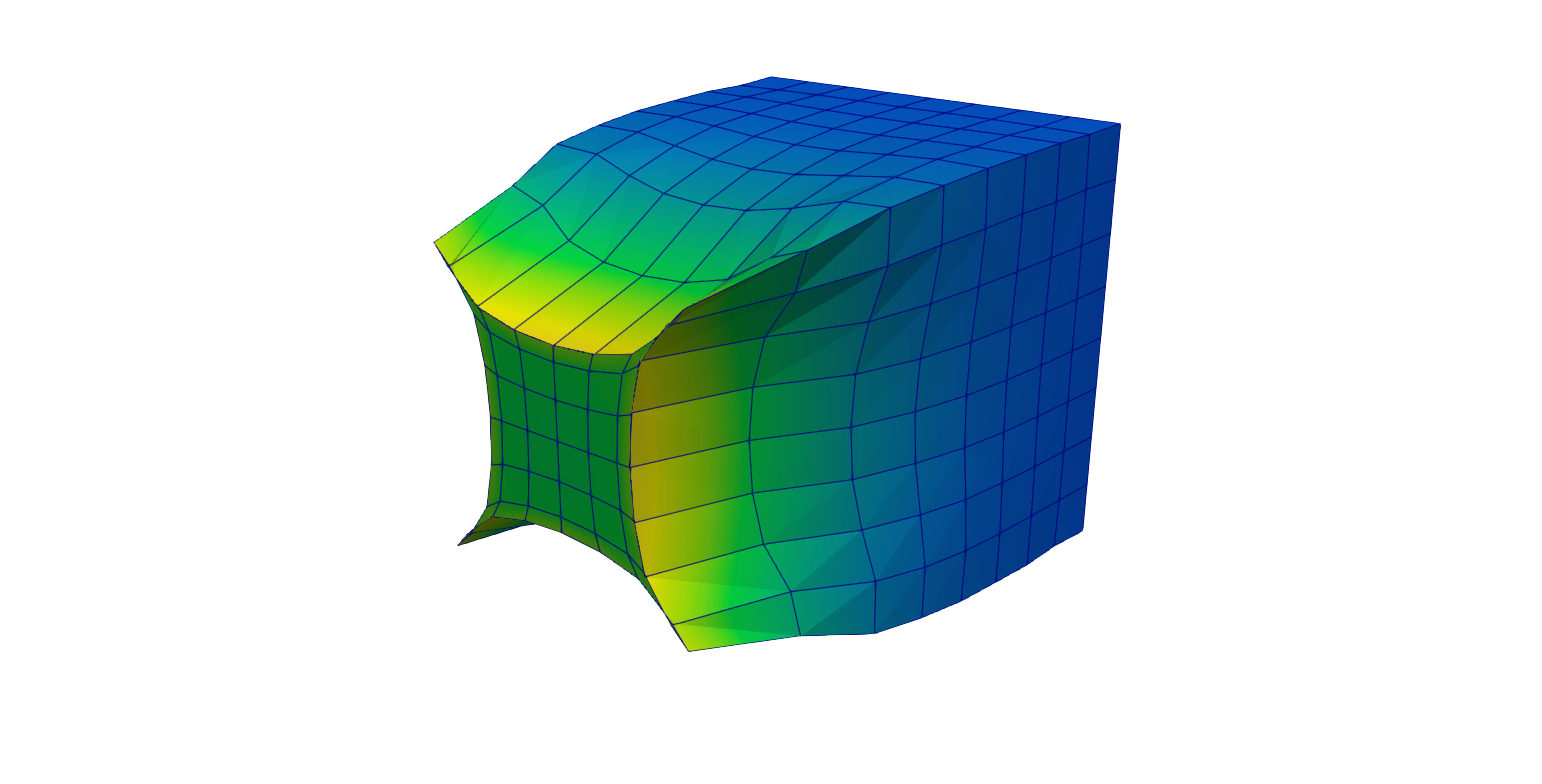
\includegraphics[height=3cm]{fig/4/4.1.5/7-1.png}
  \caption{动态显式弹塑,弹性模量210,泊松比0.3,塑性屈服0.24,体单元积分点个数为1,边界单元积分点个数为1,时间0.5,结果时间为0.25,总时间步数1000}
  \label{fig:4.1.4:4}
\end{figure}

\begin{figure}[!htbp]
  \centering
  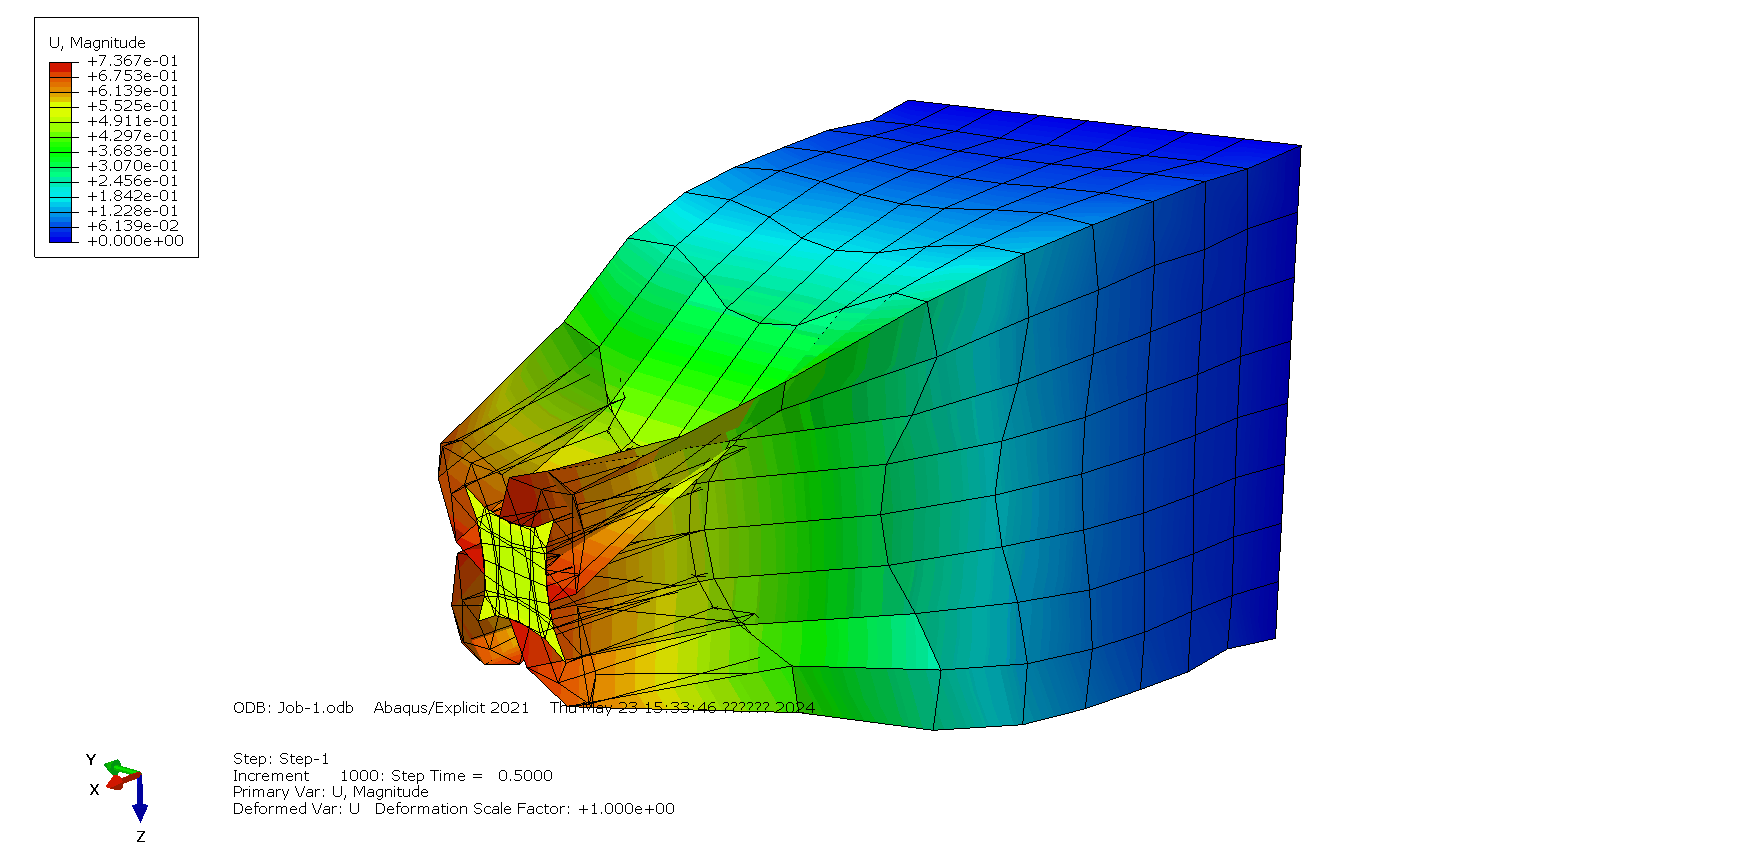
\includegraphics[height=3cm]{fig/4/4.1.5/8.png}
  \caption{动态显式弹塑,弹性模量210,泊松比0.3,塑性屈服0.24,体单元积分点个数为1,边界单元积分点个数为1,时间0.5,结果时间为0.5,总时间步数1000}
  \label{fig:4.1.4:4}
\end{figure}

\begin{figure}[!htbp]
  \centering
  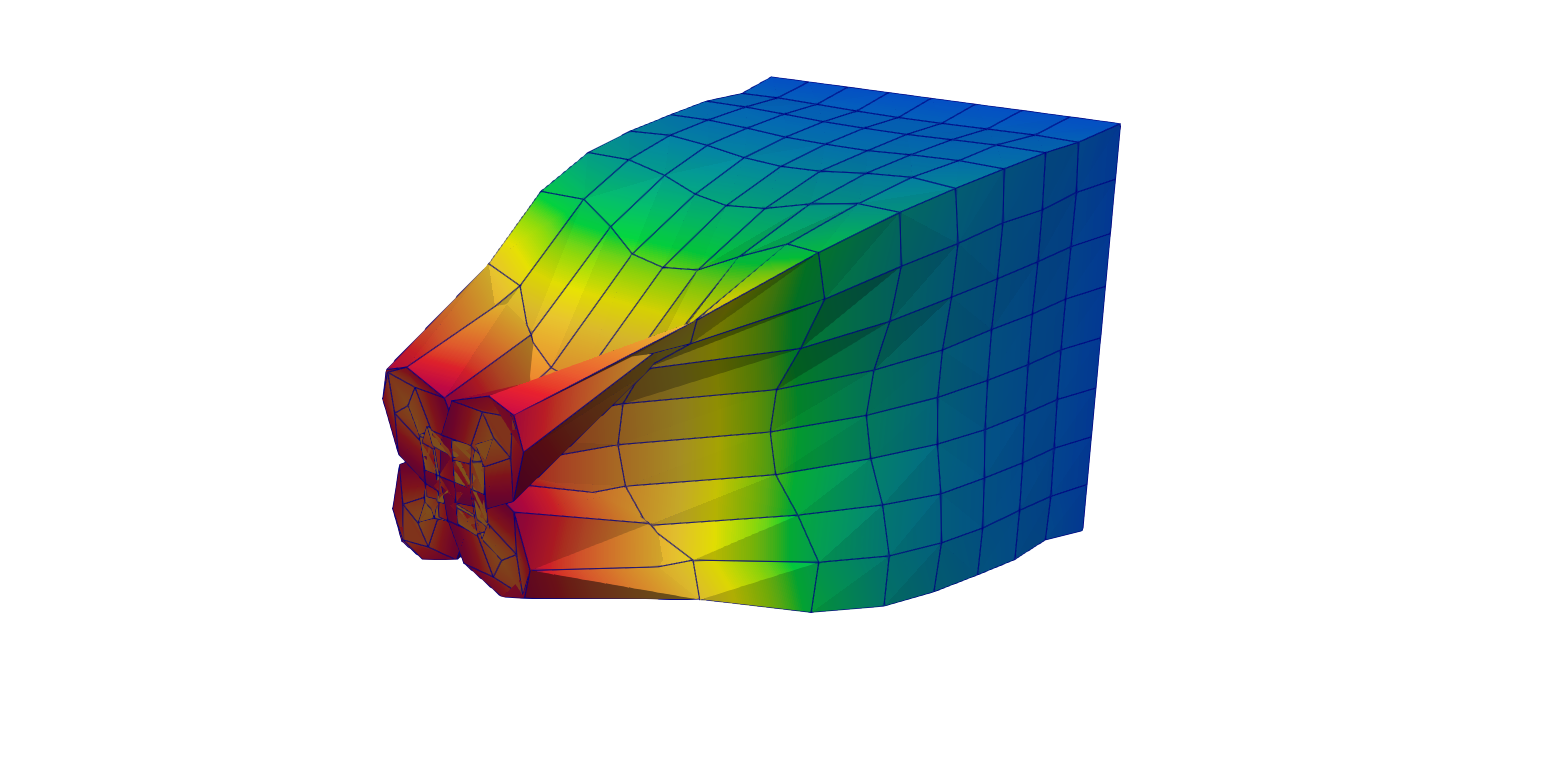
\includegraphics[height=3cm]{fig/4/4.1.5/8-1.png}
  \caption{动态显式弹塑,弹性模量210,泊松比0.3,塑性屈服0.24,体单元积分点个数为1,边界单元积分点个数为1,时间0.5,结果时间为0.5,总时间步数1000,$\max(\|\mathbf u_h\|)=0.7366931105086029$}
  \label{fig:4.1.4:4}
\end{figure}

\begin{figure}[!htbp]
  \centering
  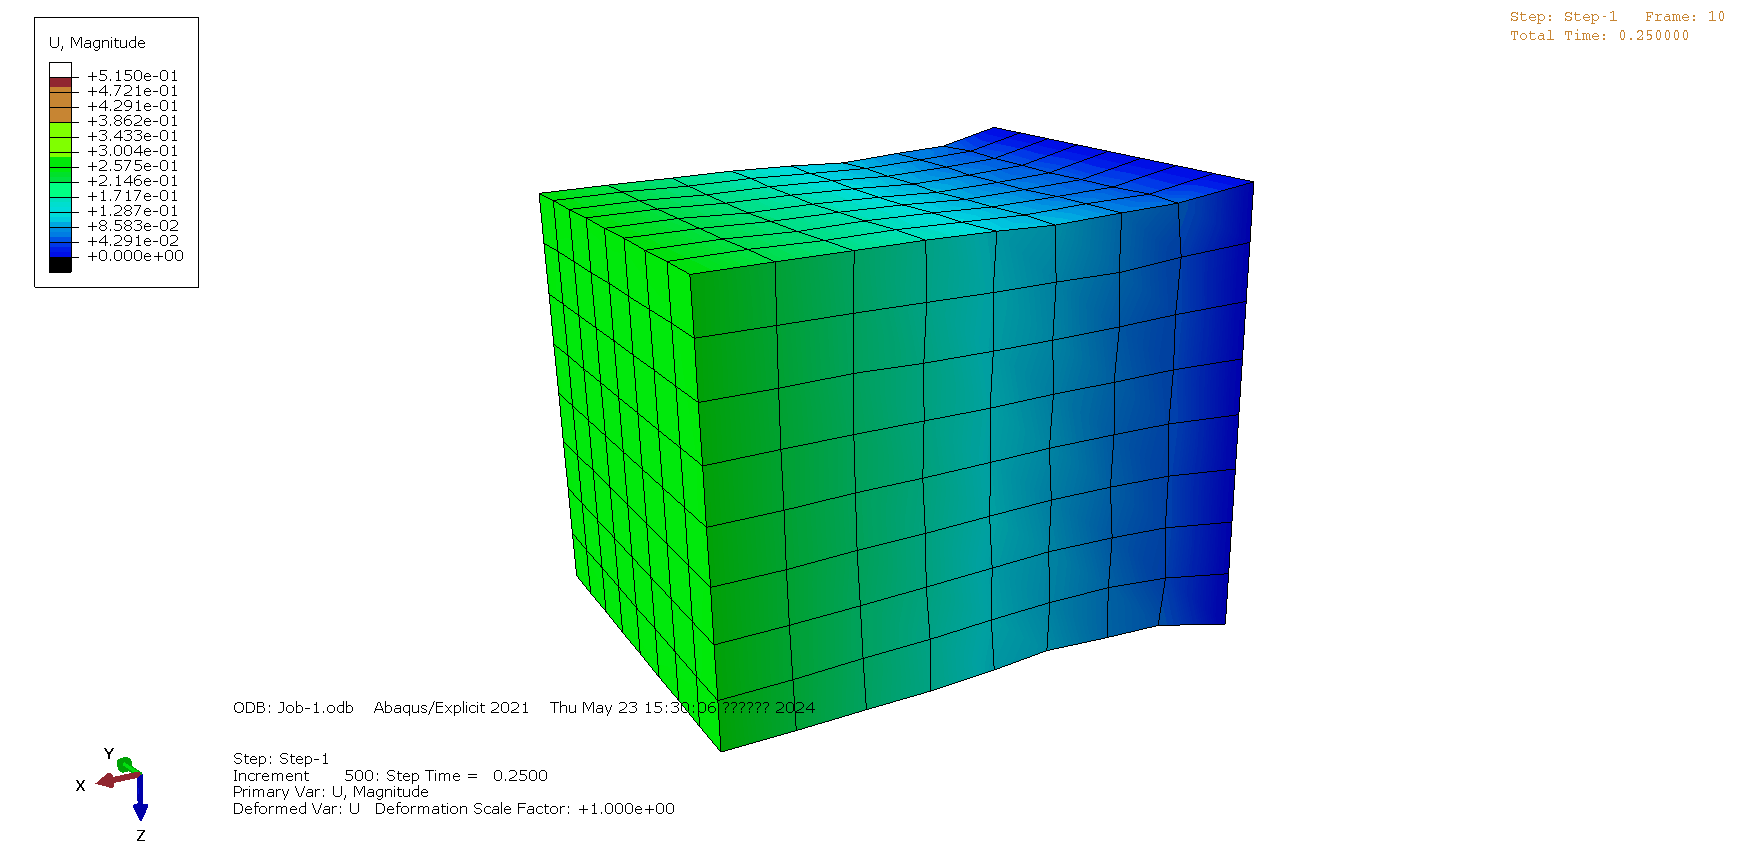
\includegraphics[height=3cm]{fig/4/4.1.5/9.png}
  \caption{动态显式弹塑,弹性模量210,泊松比0.3,塑性屈服1e10,体单元积分点个数为1,边界单元积分点个数为1,时间0.5,结果时间为0.25,总时间步数1000}
  \label{fig:4.1.4:4}
\end{figure}

\begin{figure}[!htbp]
  \centering
  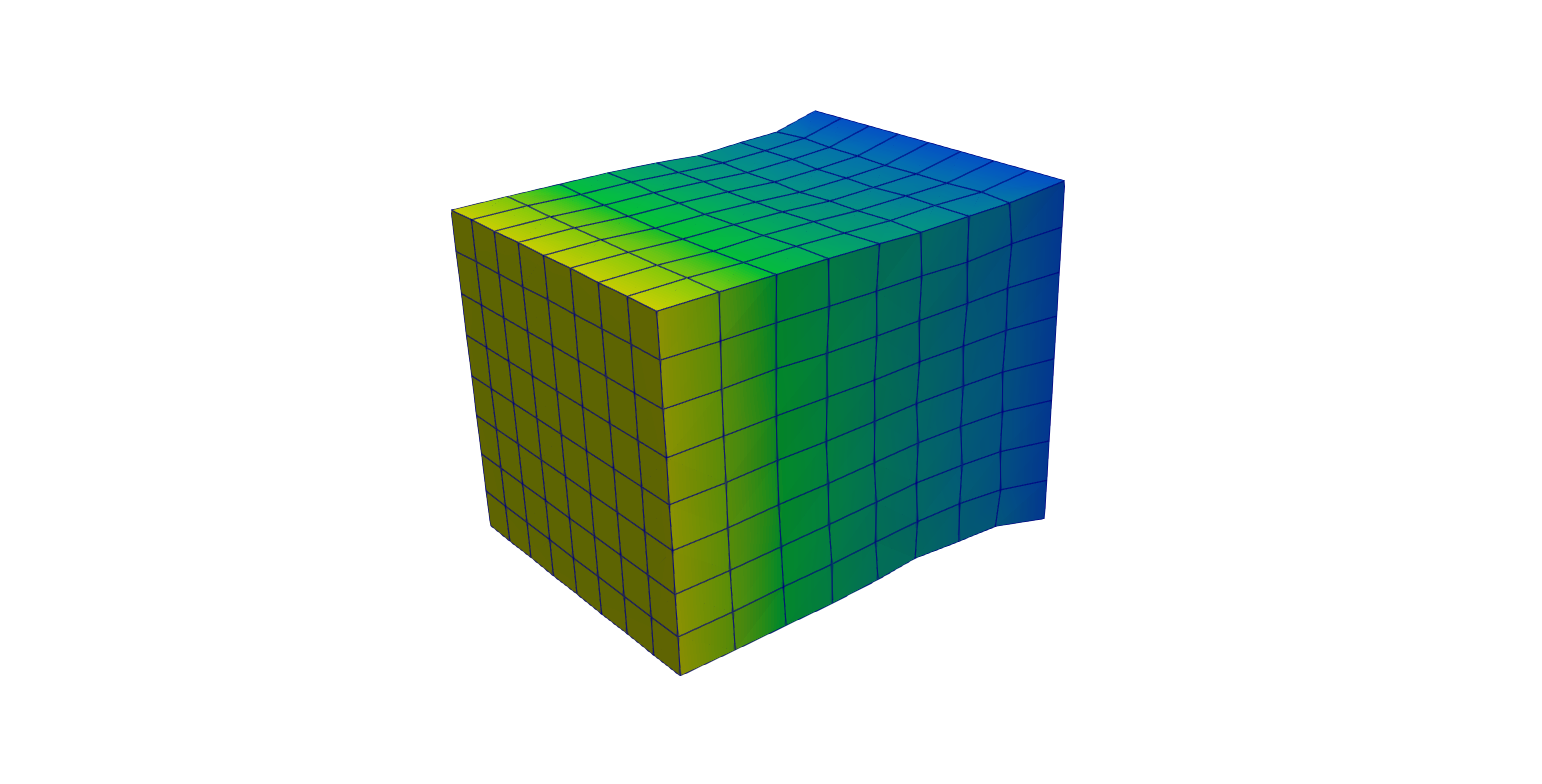
\includegraphics[height=3cm]{fig/4/4.1.5/9-1.png}
  \caption{动态显式弹塑,弹性模量210,泊松比0.3,塑性屈服1e10,体单元积分点个数为1,边界单元积分点个数为1,时间0.5,结果时间为0.25,总时间步数1000}
  \label{fig:4.1.4:4}
\end{figure}

\begin{figure}[!htbp]
  \centering
  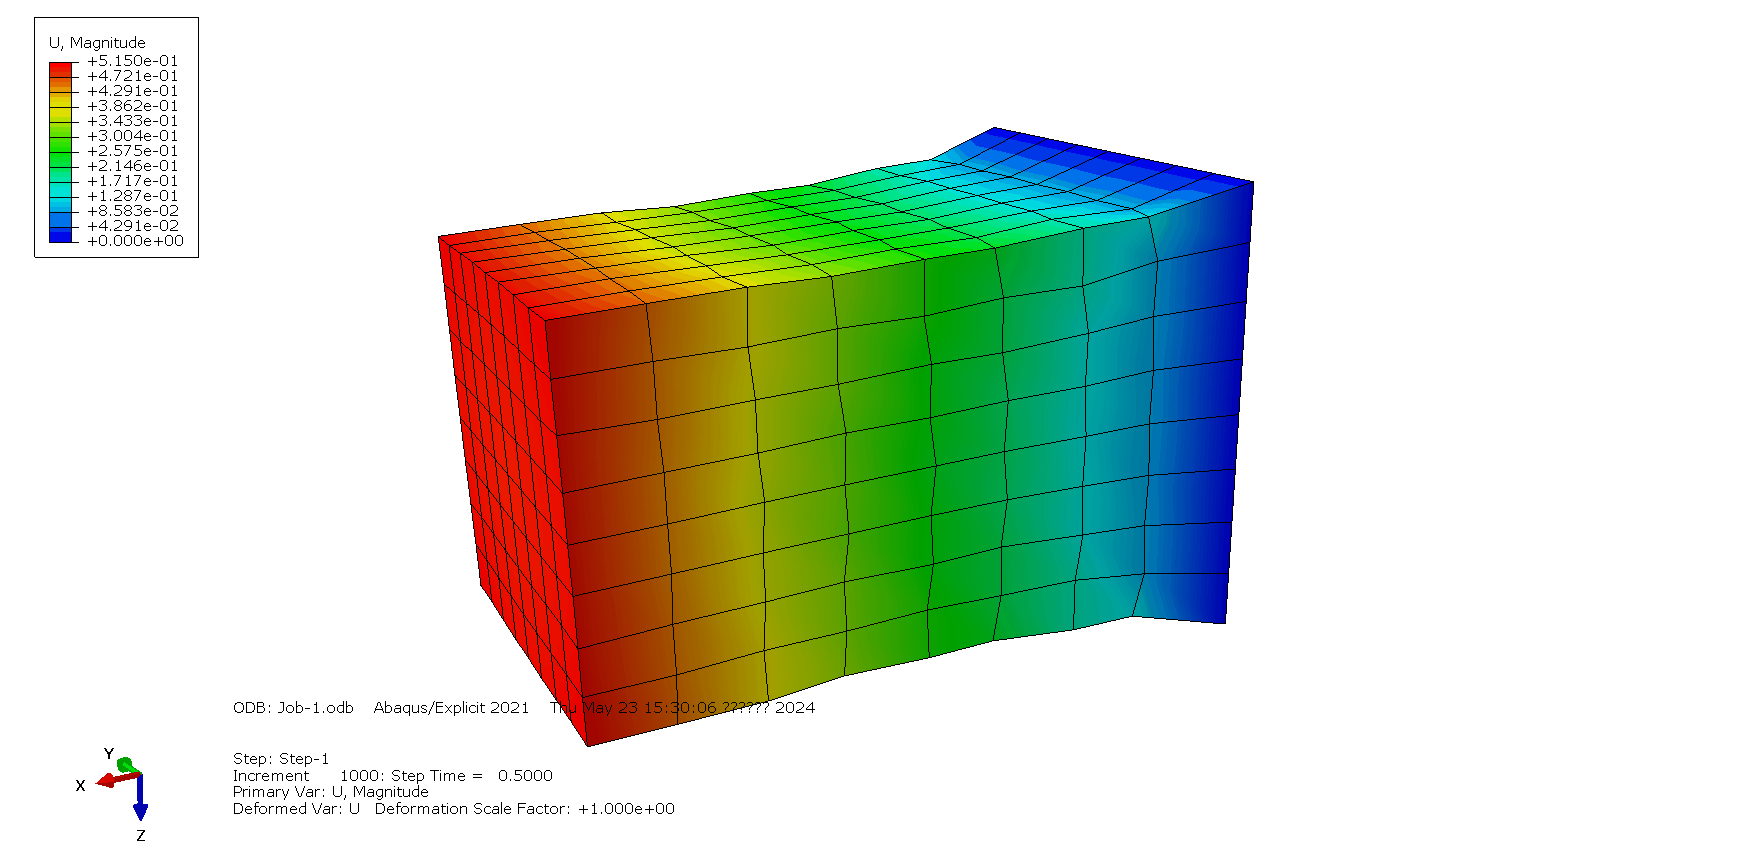
\includegraphics[height=3cm]{fig/4/4.1.5/10.png}
  \caption{动态显式弹塑,弹性模量210,泊松比0.3,塑性屈服1e10,体单元积分点个数为1,边界单元积分点个数为1,时间0.5,结果时间为0.5,总时间步数1000}
  \label{fig:4.1.4:4}
\end{figure}

\begin{figure}[!htbp]
  \centering
  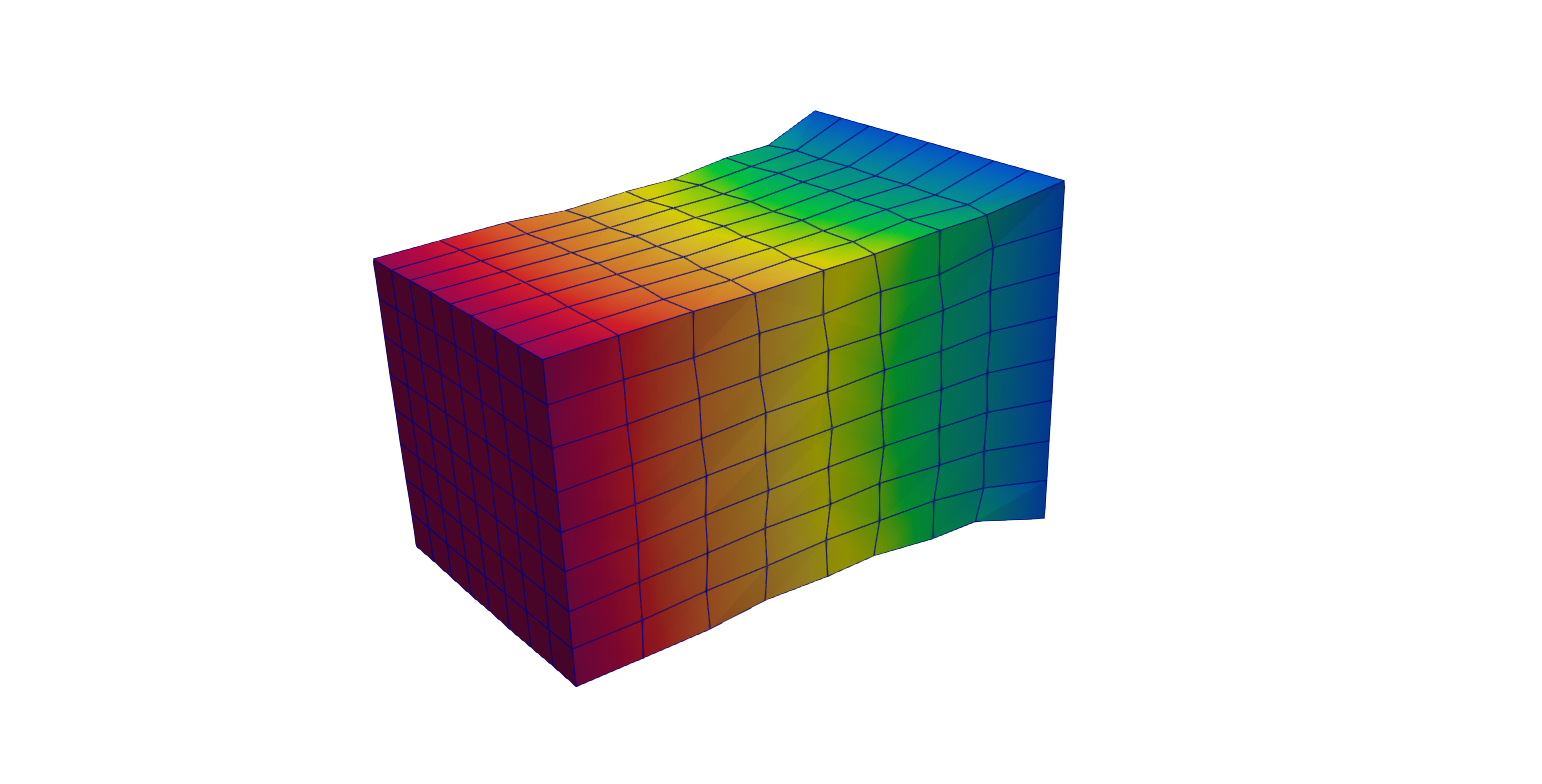
\includegraphics[height=3cm]{fig/4/4.1.5/10-1.png}
  \caption{动态显式弹塑,弹性模量210,泊松比0.3,塑性屈服1e10,体单元积分点个数为1,边界单元积分点个数为1,时间0.5,结果时间为0.5,总时间步数1000}
  \label{fig:4.1.4:4}
\end{figure}


\newpage
\subsection{热弹塑性}


首先定义热弹性问题。这里需要注意的是方程中$\mathbf\sigma$不是全部应力,是去掉温度场影响后的应力。

\begin{align*}
  & -\nabla\cdot\mathbf \sigma = \mathbf b \\
  & \rho c\frac{\ud T}{\ud t} + \nabla\cdot \left(\mathbf K \nabla T\right)  = r\\
  & \varepsilon_T = \alpha(T-T_0)\delta_{ij} \\
  &\mathbf\sigma = \mathbf D(\mathbf\varepsilon-\mathbf\varepsilon_T)
\end{align*}

\begin{align*}
  \mathbf\sigma =& \mathbf D(\mathbf\varepsilon-\mathbf\varepsilon_T)\\
  =&2\mu(\mathbf\varepsilon-\mathbf\varepsilon_T) + \lambda\mathrm{tr}(\mathbf \varepsilon-\mathbf\varepsilon_T)\mathbf 1\\
  =&2\mu\mathbf\varepsilon + \lambda\mathrm{tr}(\mathbf \varepsilon)\mathbf 1 - 2\mu\mathbf\varepsilon_T - \lambda\mathrm{tr}(\mathbf\varepsilon_T)\mathbf 1\\
  =&2\mu\mathbf\varepsilon + \lambda\mathrm{tr}(\mathbf \varepsilon)\mathbf 1 - 2\mu\mathbf\varepsilon_T - \lambda3\alpha (T-T_0)\mathbf 1
\end{align*}

\begin{align*}
  -\int_{\Omega}\nabla\cdot\mathbf \sigma\cdot\mathbf v\ud x =& \int_{\Omega}\mathbf b\cdot\mathbf v\ud x \\
  -\int_{\Gamma}\mathbf\sigma\cdot\mathbf n\cdot\mathbf v\ud s_x      +\int_{\Omega}\mathbf\sigma:\mathbf\varepsilon(\mathbf v)\ud x =& \int_{\Omega}\mathbf b\cdot\mathbf v\ud x\\
  \int_{\Omega}\left(2\mu\mathbf \varepsilon(\mathbf u) :\mathbf\varepsilon(\mathbf v)+\lambda\nabla\cdot\mathbf u \nabla\cdot\mathbf v\right)\ud x =&
  \int_{\Gamma} \alpha(T-T_0)(3\lambda+2\mu)\mathbf 1:\mathbf\varepsilon(\mathbf v)\ud x + \int_{\Gamma}\mathbf t\cdot\mathbf v\ud s_x + \int_{\Omega}\mathbf b\cdot\mathbf v\ud x
\end{align*}

\begin{align*}
   \int_{\Omega}(-\nabla\cdot(2\mu\mathbf\varepsilon + \lambda\mathrm{tr}(\mathbf \varepsilon)\mathbf 1))\cdot\mathbf v \ud x
   = \int_{\Omega}\mathbf b\cdot\mathbf v\ud x  + \int_{\Omega} T\nabla\cdot\mathbf v \ud x - \int_{\Gamma}\mathbf n\cdot\mathbf v T\ud s_x
\end{align*}

\begin{align*}
  \int_{\Omega}\frac{\ud T}{\ud t}v\ud x - \int_{\Omega}\nabla\cdot \left(\nabla T\right)v\ud x   =& \int_{\Omega}rv\ud x \\
  \int_{\Omega}\frac{\ud T}{\ud t}v\ud x + \int_{\Omega}\nabla T\cdot\nabla v\ud x   =& \int_{\Omega}rv\ud x + \int_{\Gamma}\mathbf n\cdot\nabla T v\ud s_x
\end{align*}


  
热应力2D和Abaqus比较,杨氏模量为2.5,泊松比为0.25,热传导为1,比热为1,密度为1,膨胀系数为1,底部固定,上边温度为1,左右下边热流为0,上边方向向上拖拽力为0.1。  

\begin{figure}[!htbp]
  \centering
  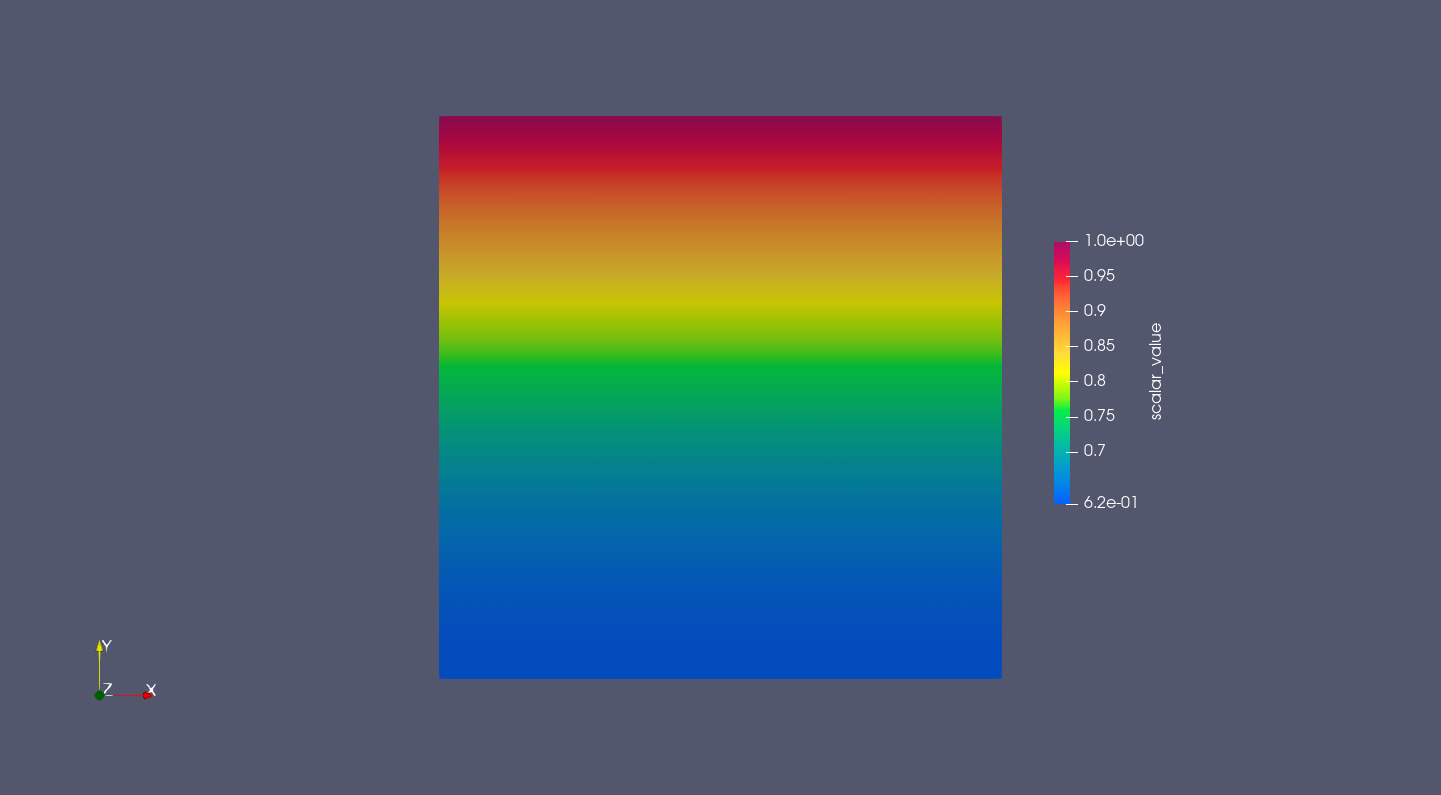
\includegraphics[height=3cm]{fig/4/3.10.5:1.png}
  \caption{$T$,level 5-6,$\mathrm{time}=0.5$, $T_{\max}=0.6247779726982117$}
  \label{fig:4.1.4:4}
\end{figure}

\begin{figure}[!htbp]
  \centering
  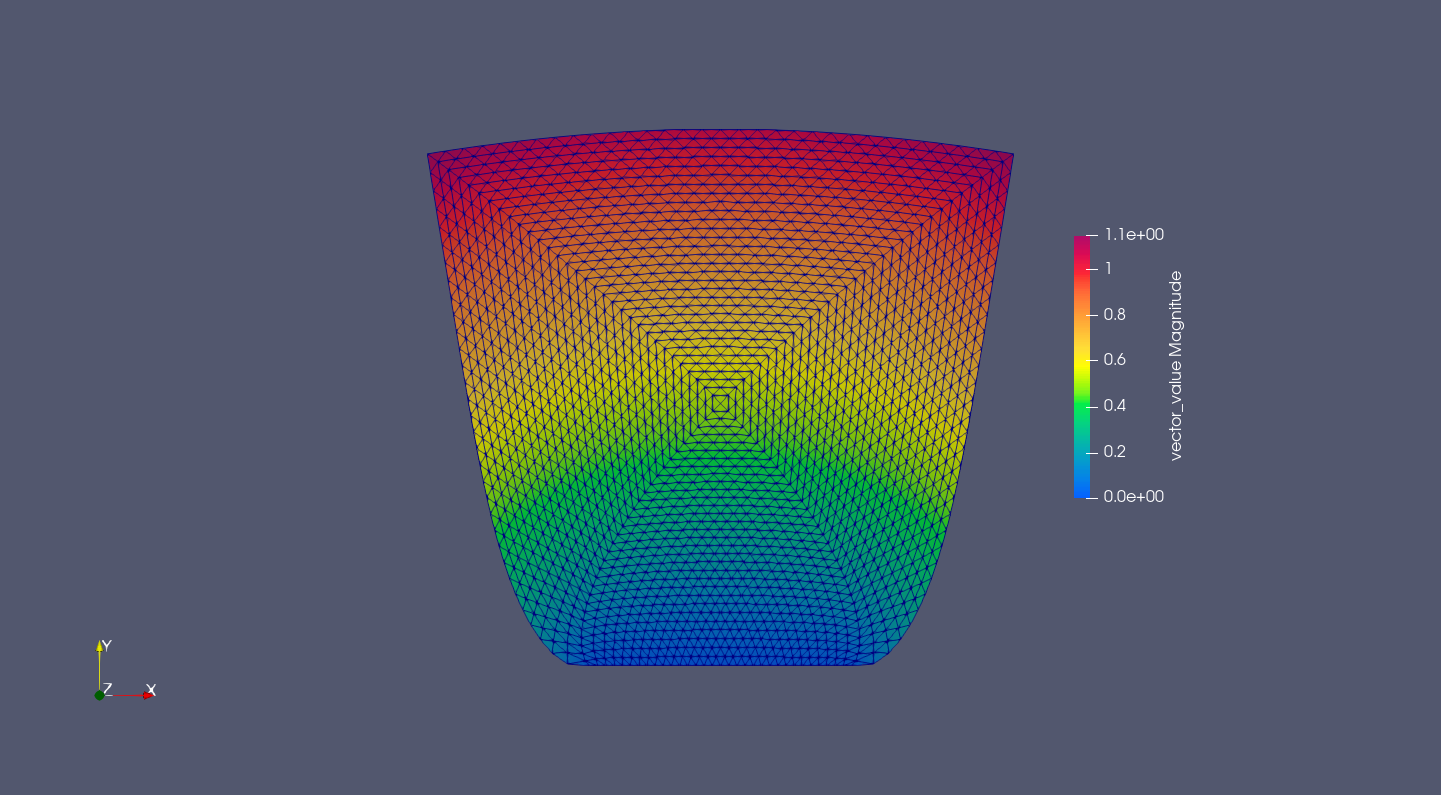
\includegraphics[height=3cm]{fig/4/3.10.5:2.png}
  \caption{$T$,level 5-6,$\mathrm{time}=0.5$,$\|\mathbf u\|_{\max}=1.1456380793904821$}
  \label{fig:4.1.4:4}
\end{figure}

\begin{figure}[!htbp]
  \centering
  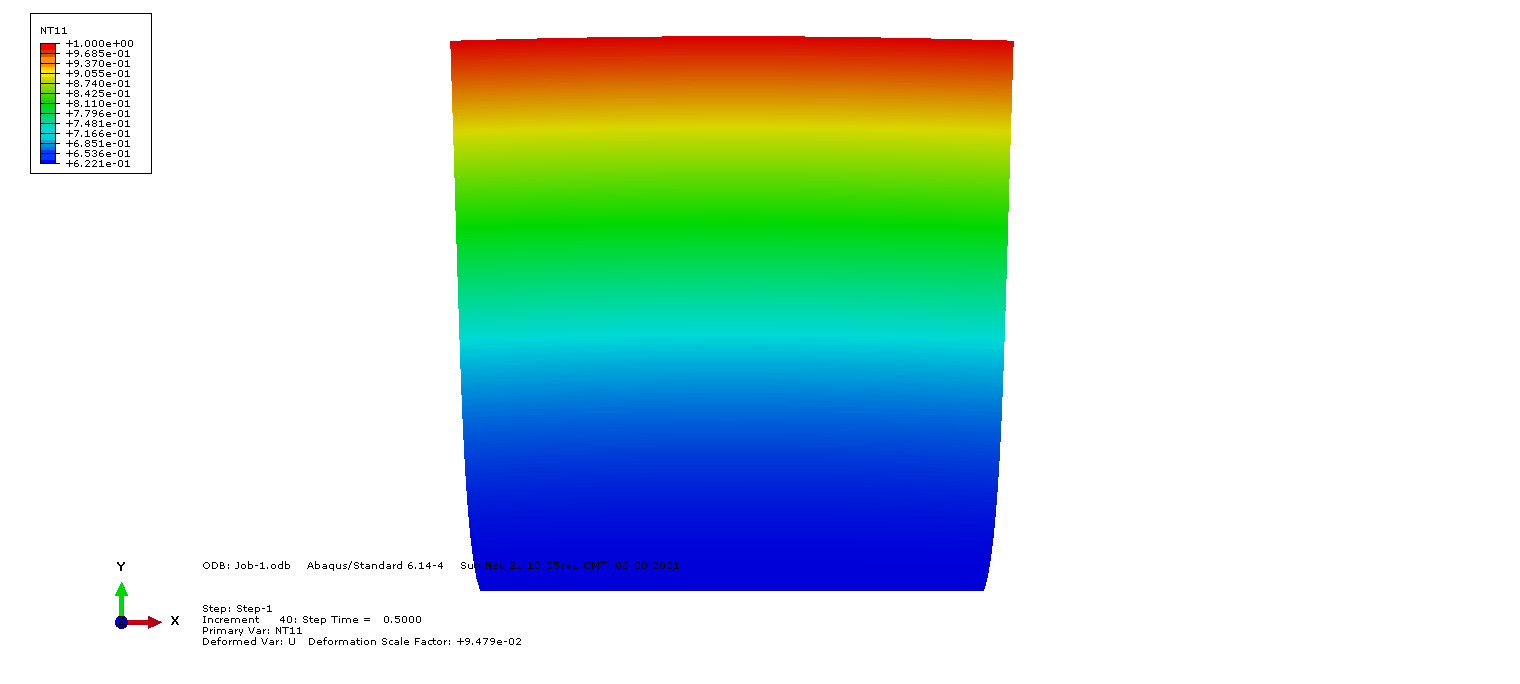
\includegraphics[height=3cm]{fig/4/3.10.5:3.png}
  \caption{$T$,$h=0.025$,$k=0.0125$,$\mathrm{time}=0.5$,$T_{\max}=6.221\mathrm e-01$}
  \label{fig:4.1.4:4}
\end{figure}

\begin{figure}[!htbp]
  \centering
  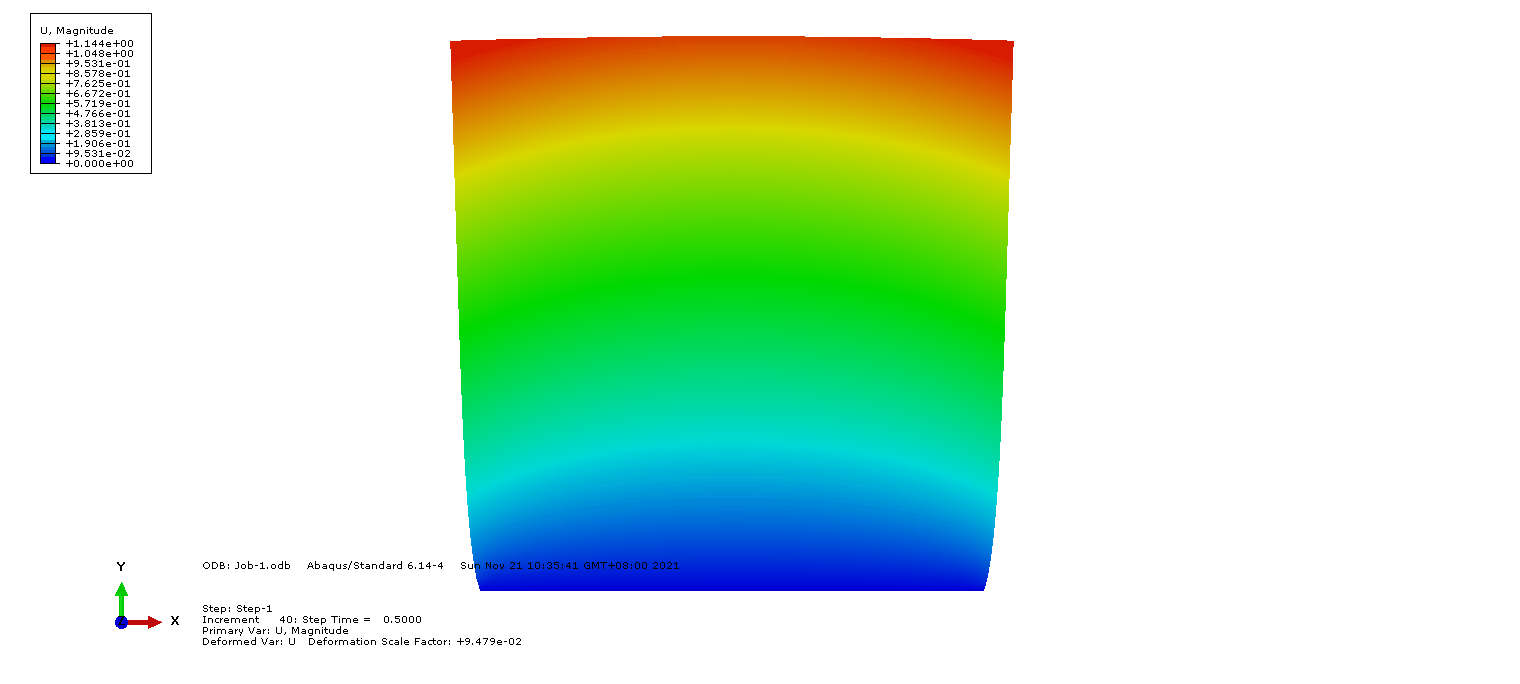
\includegraphics[height=3cm]{fig/4/3.10.5:4.png}
  \caption{$T$,$h=0.025$,$k=0.0125$,$\mathrm{time}=0.5$,$\|\mathbf u\|_{\max}=1.144$}
  \label{fig:4.1.4:4}
\end{figure}

热应力3D和Abaqus比较,杨氏模量为2.5,泊松比为0.25,热传导为1,比热为1,密度为1,膨胀系数为1,底部固定,上边温度为1,左右下边热流为0,上边方向向上拖拽力为0.1。  

\begin{figure}[!htbp]
  \centering
  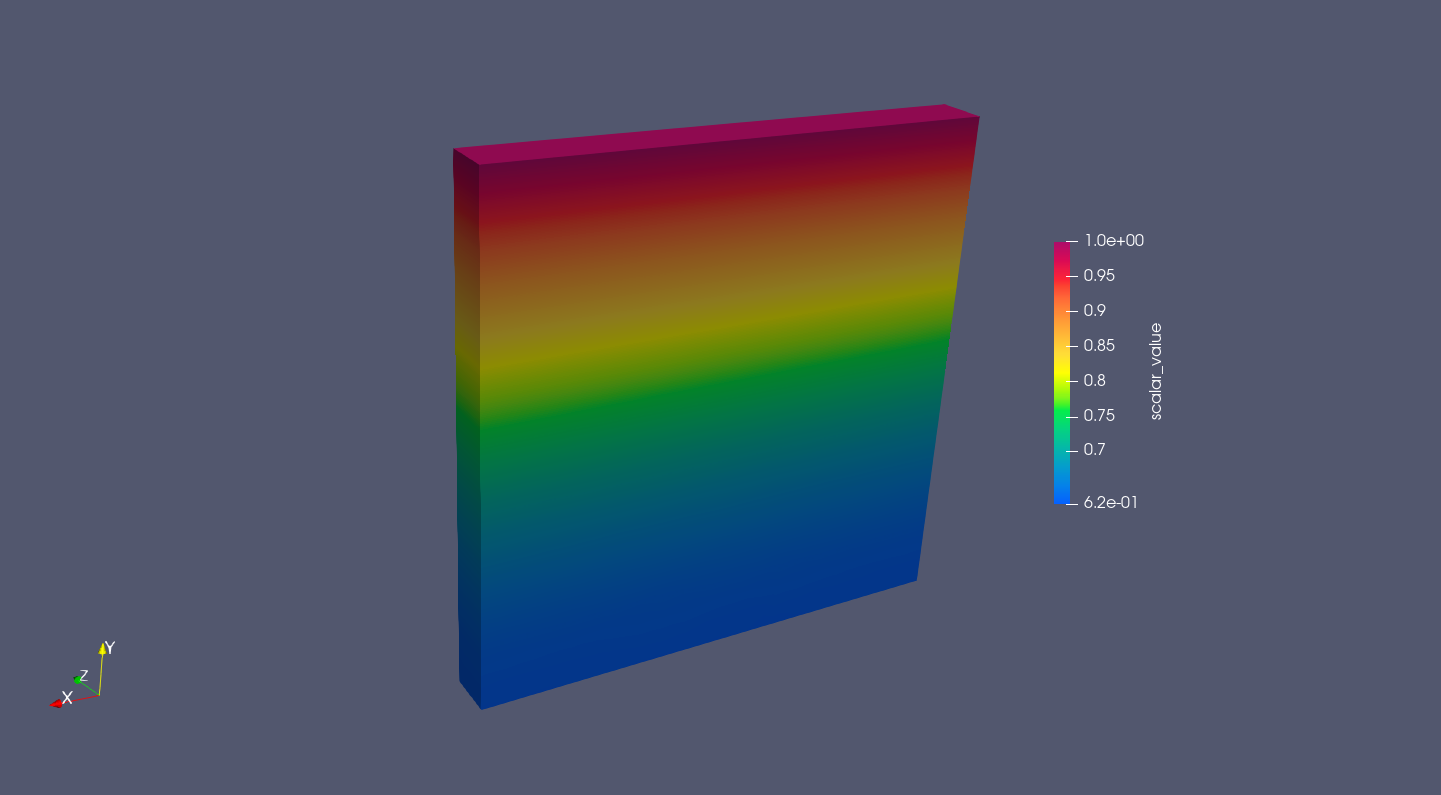
\includegraphics[height=3cm]{fig/4/3.10.5:5.png}
  \caption{$T$,level 0-6,$\mathrm{time}=0.5$,$T_{\max}=0.6236979961395264$}
  \label{fig:4.1.4:4}
\end{figure}

\begin{figure}[!htbp]
  \centering
  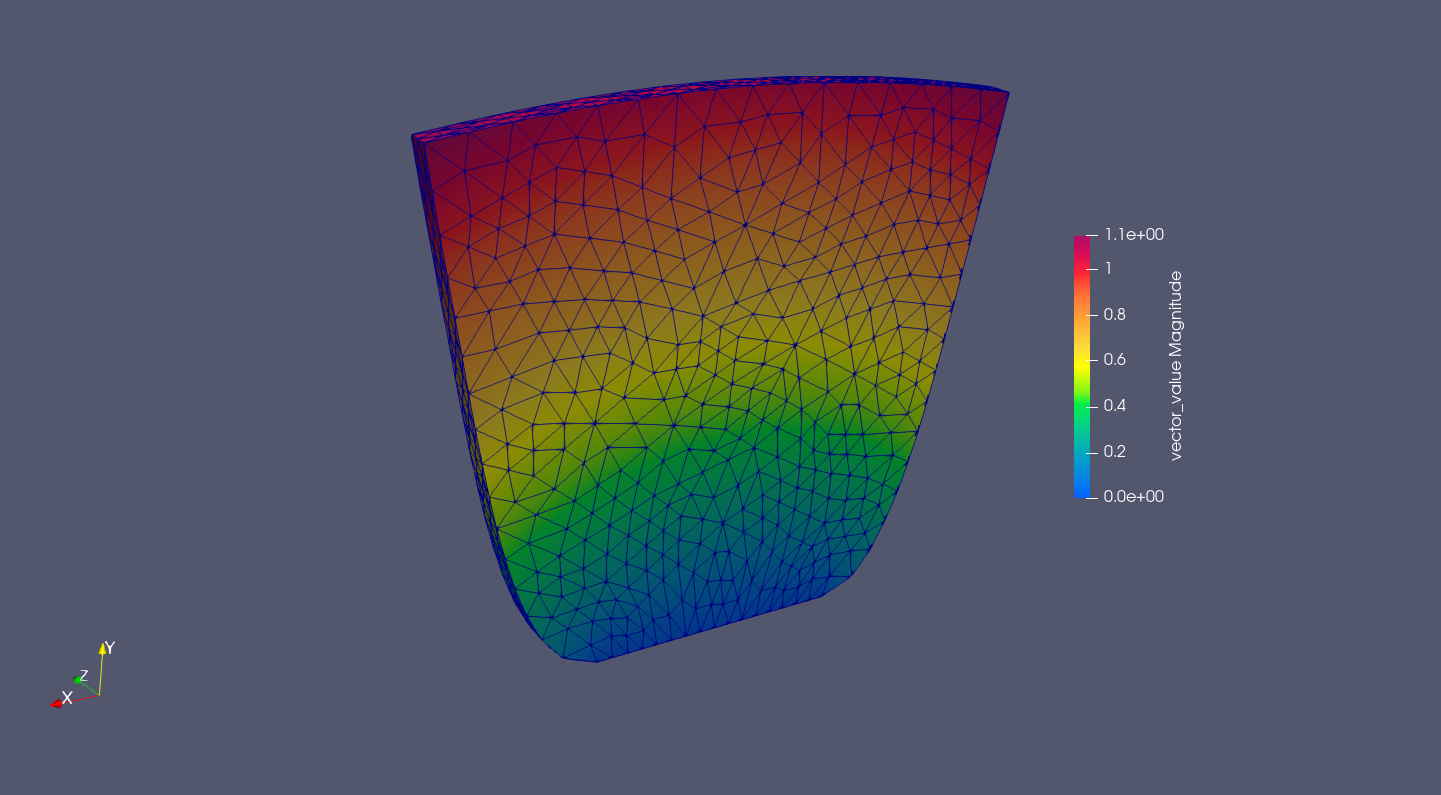
\includegraphics[height=3cm]{fig/4/3.10.5:6.png}
  \caption{$T$,level 5-6,$\mathrm{time}=0.5$,$\|\mathbf u\|_{\max}=1.1469914204042906$}
  \label{fig:4.1.4:4}
\end{figure}

\begin{figure}[!htbp]
  \centering
  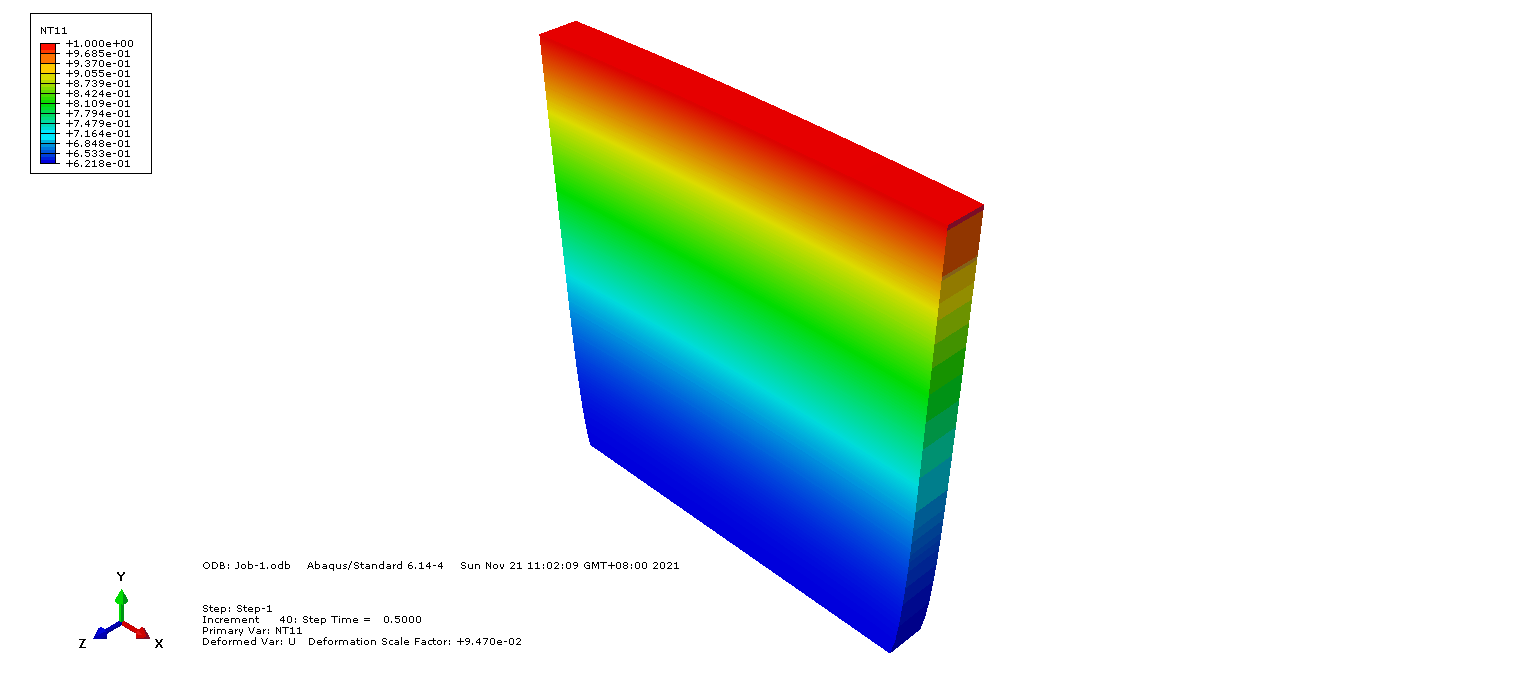
\includegraphics[height=3cm]{fig/4/3.10.5:7.png}
  \caption{$T$,$h=0.05$,$k=0.0125$,$\mathrm{time}=0.5$,$T_{\max}=6.218\mathrm e-01$}
  \label{fig:4.1.4:4}
\end{figure}

\begin{figure}[!htbp]
  \centering
  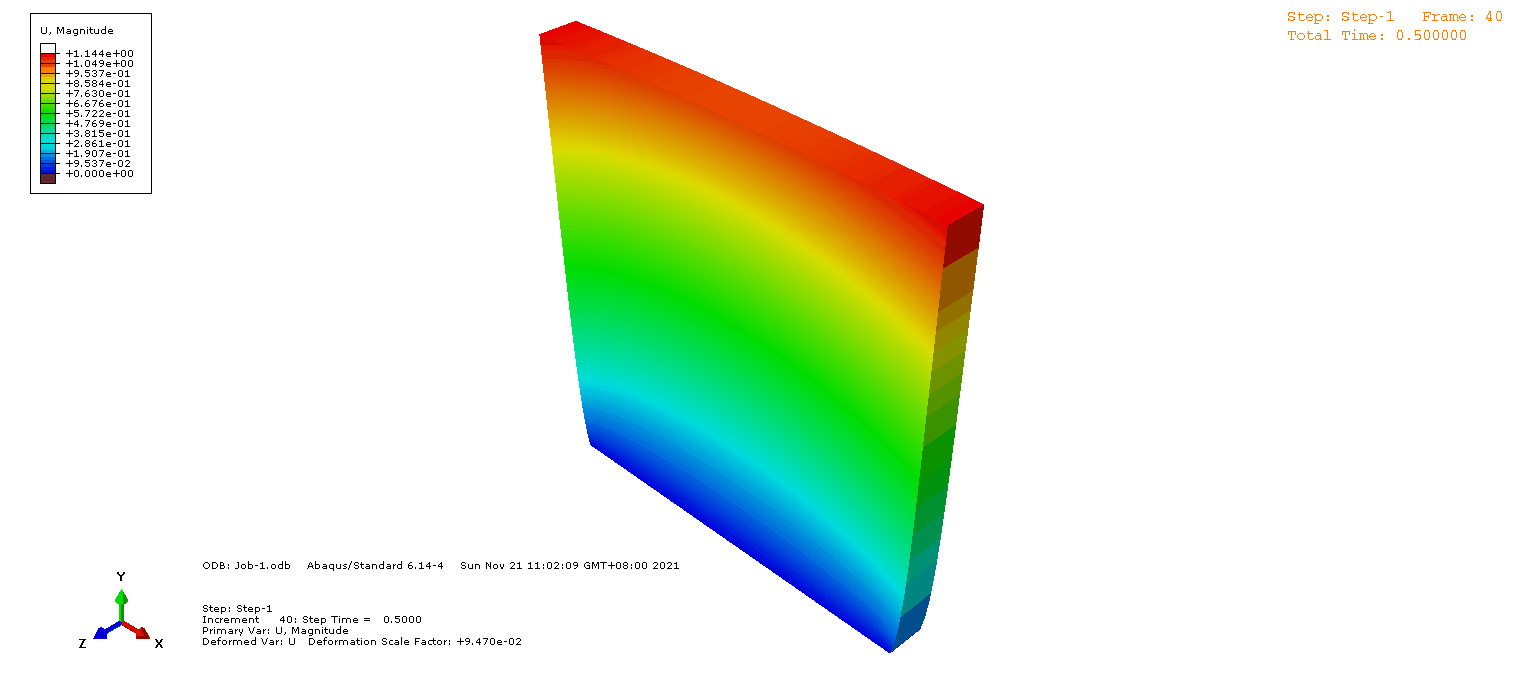
\includegraphics[height=3cm]{fig/4/3.10.5:8.png}
  \caption{$T$,$h=0.05$,$k=0.0125$,$\mathrm{time}=0.5$,$\|\mathbf u\|_{\max}=1.144$}
  \label{fig:4.1.4:4}
\end{figure}


其次对于热弹塑性问题,屈服准则受到温度影响,例如理想塑性的屈服准则,$\sigma_\theta$是温度的函数。

\begin{align*}	   
  f = \mathbf S:\mathbf S-\frac{2}{3}\sigma^2_\theta
\end{align*}

\begin{figure}[!htbp]
  \centering
  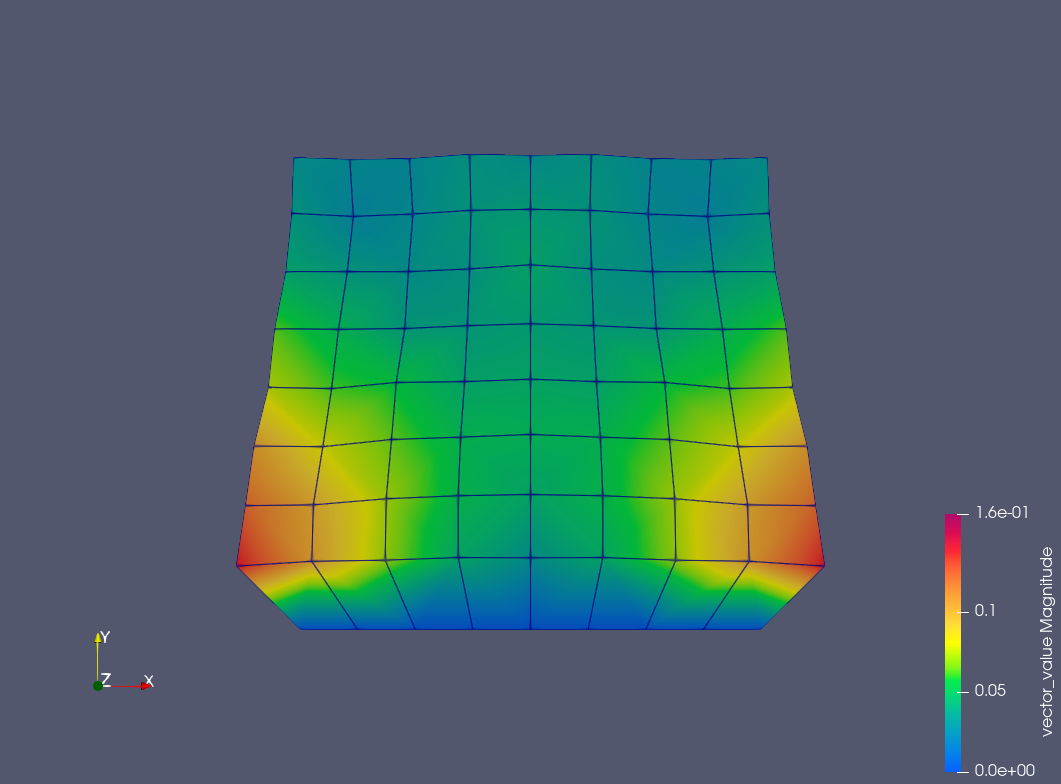
\includegraphics[height=3cm]{fig/4/4.1.6/4.1.6.3.png}
  \caption{热传导为1,比热为1,热膨胀为1,需要注意如果不设置热膨胀,温度场和弹塑性无法耦合,弹性模量为210,泊松比为0.3,屈服应力为0.24,时间长度为0.5,时间步数为1000,0.16112902009654156}
  \label{fig:4.1.4:4}
\end{figure}

\begin{figure}[!htbp]
  \centering
  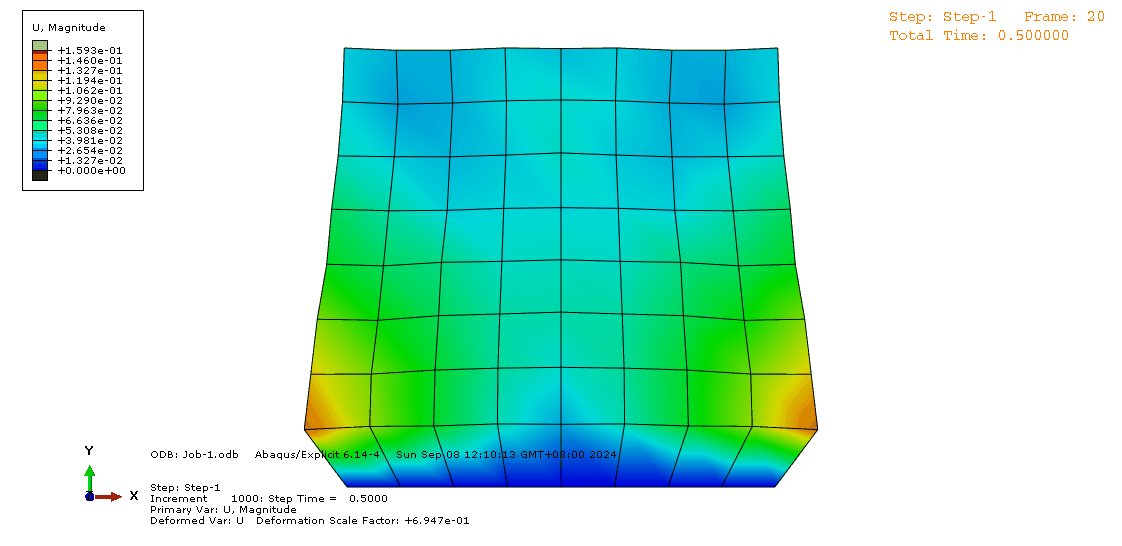
\includegraphics[height=3cm]{fig/4/4.1.6/4.1.6.4.png}
  \caption{热传导为1,比热为1,热膨胀为1,需要注意如果不设置热膨胀,温度场和弹塑性无法耦合,弹性模量为210,泊松比为0.3,屈服应力为0.24,时间长度为0.5,时间步数为1000,Abaqus里需要将求解器和网格单元都设置成温度场和位移场耦合}
  \label{fig:4.1.4:4}
\end{figure}

\begin{figure}[!htbp]
  \centering
  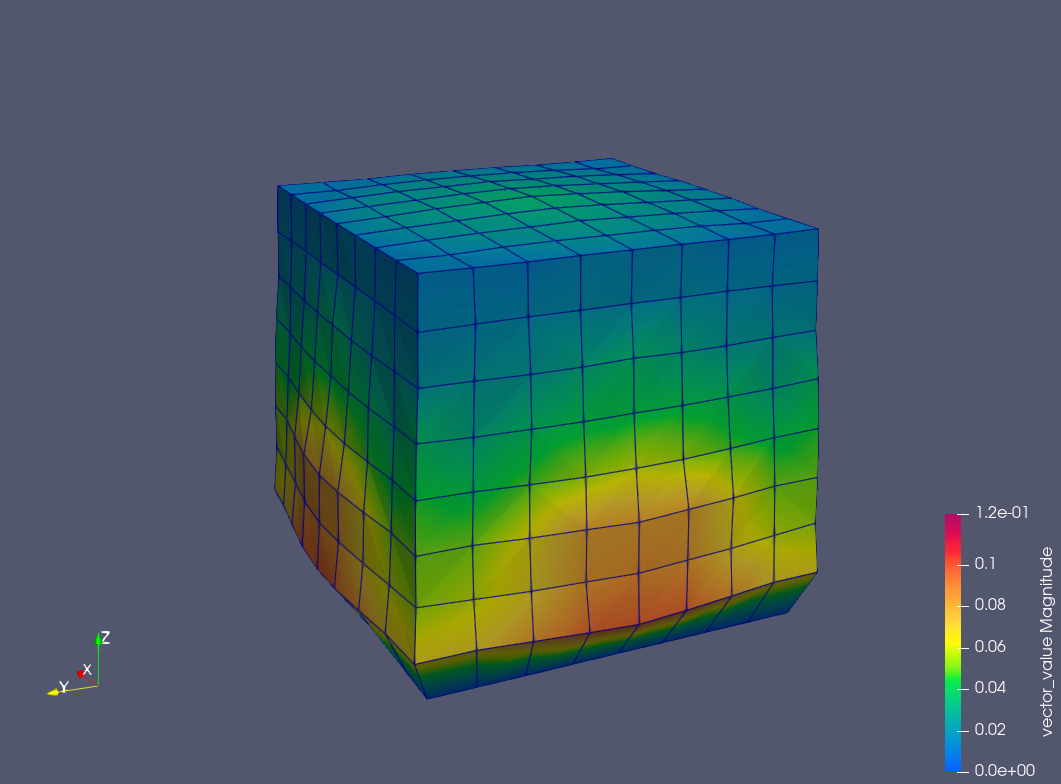
\includegraphics[height=3cm]{fig/4/4.1.6/4.1.6.1.png}
  \caption{热传导为1,比热为1,热膨胀为1,需要注意如果不设置热膨胀,温度场和弹塑性无法耦合,弹性模量为210,泊松比为0.3,屈服应力为0.24,时间长度为0.5,时间步数为1000,0.12430641816539166}
  \label{fig:4.1.4:4}
\end{figure}

\begin{figure}[!htbp]
  \centering
  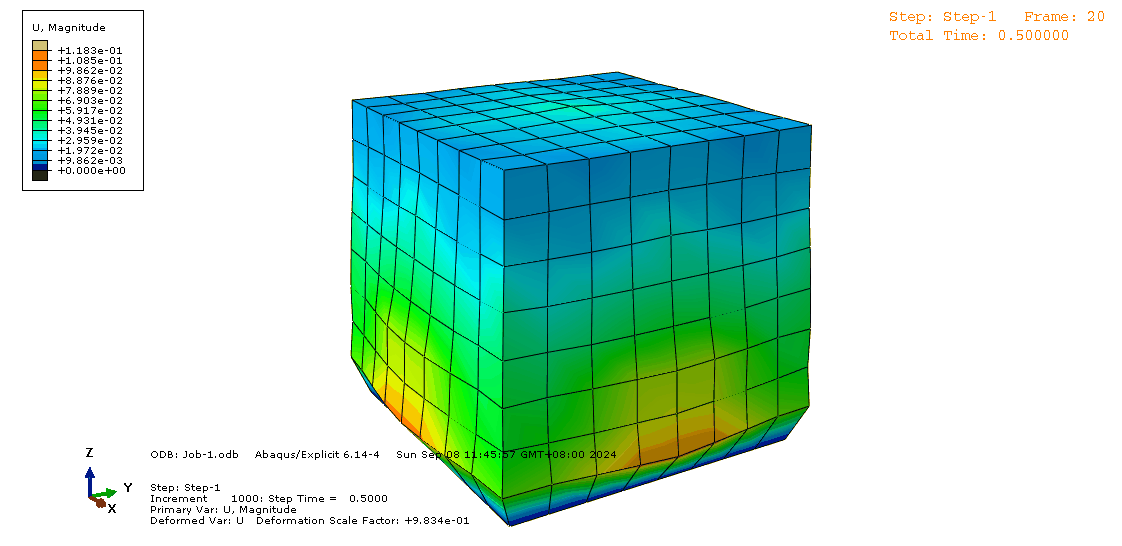
\includegraphics[height=3cm]{fig/4/4.1.6/4.1.6.2.png}
  \caption{热传导为1,比热为1,热膨胀为1,需要注意如果不设置热膨胀,温度场和弹塑性无法耦合,弹性模量为210,泊松比为0.3,屈服应力为0.24,时间长度为0.5,时间步数为1000,Abaqus里需要将求解器和网格单元都设置成温度场和位移场耦合}
  \label{fig:4.1.4:4}
\end{figure}


\newpage
\subsection{热循环计算}

\begin{figure}[!htbp]
  \centering
  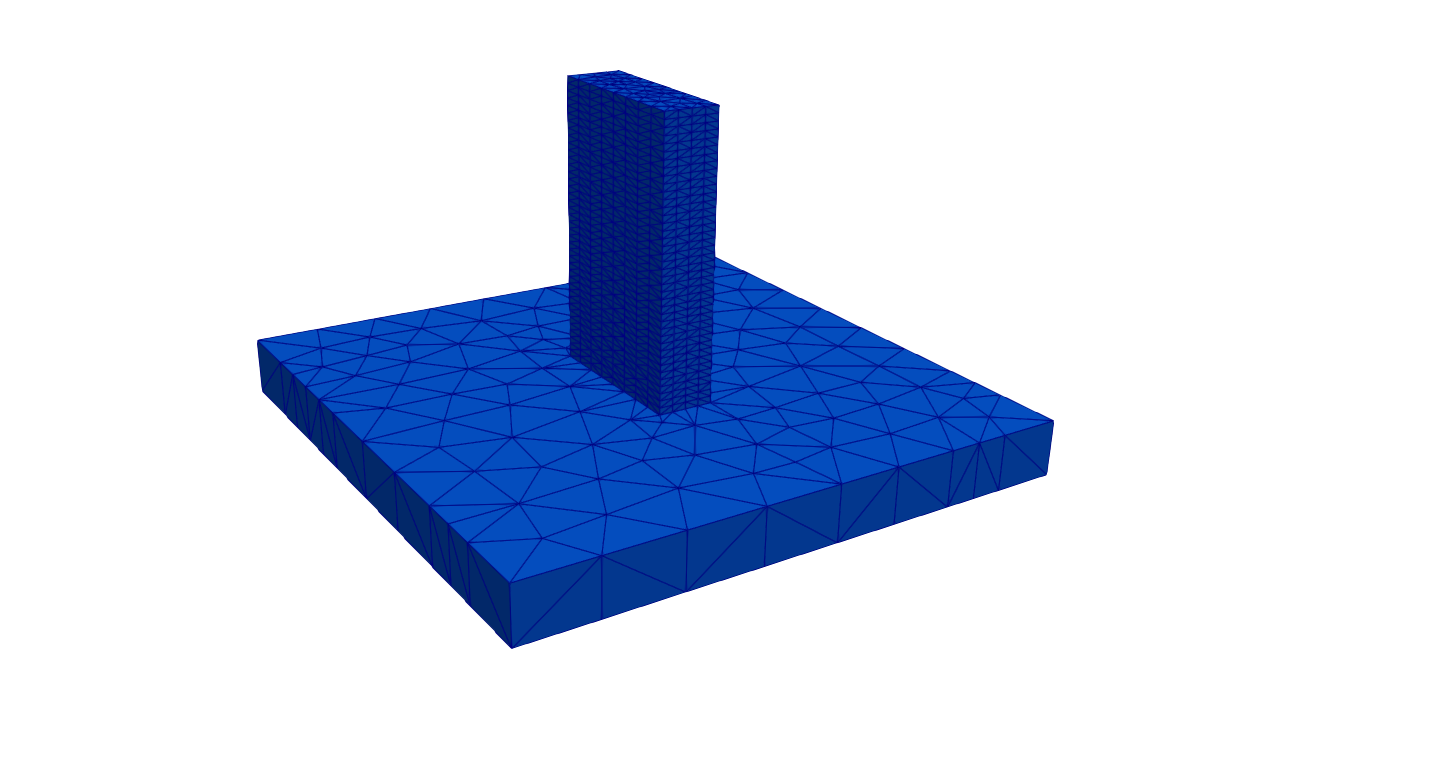
\includegraphics[height=3cm]{fig/4/4.1.6/4.1.6.11.png}
  \caption{时间为0,温度场}
  \label{fig:4.1.4:4}
\end{figure}

\begin{figure}[!htbp]
  \centering
  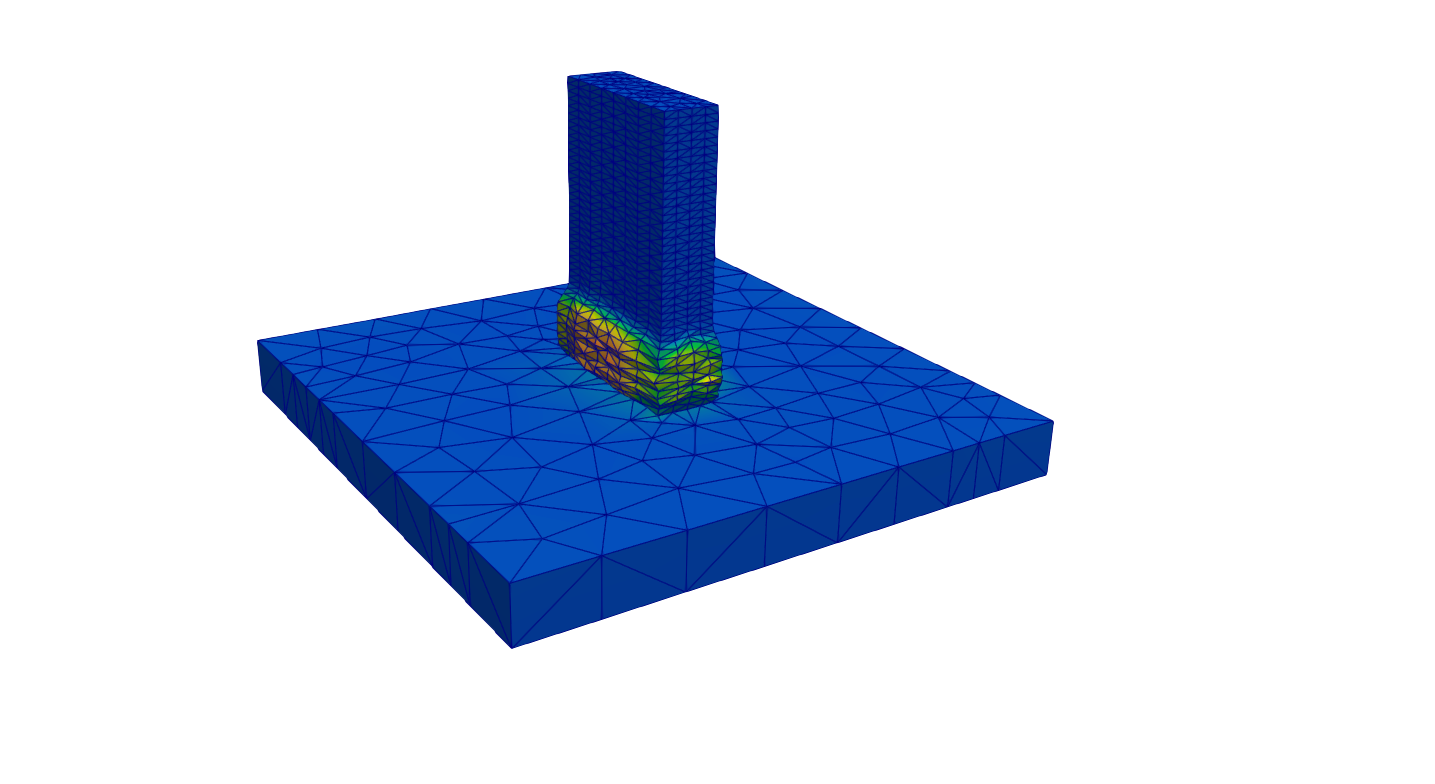
\includegraphics[height=3cm]{fig/4/4.1.6/4.1.6.12.png}
  \caption{时间为0.3,温度场}
  \label{fig:4.1.4:4}
\end{figure}

\begin{figure}[!htbp]
  \centering
  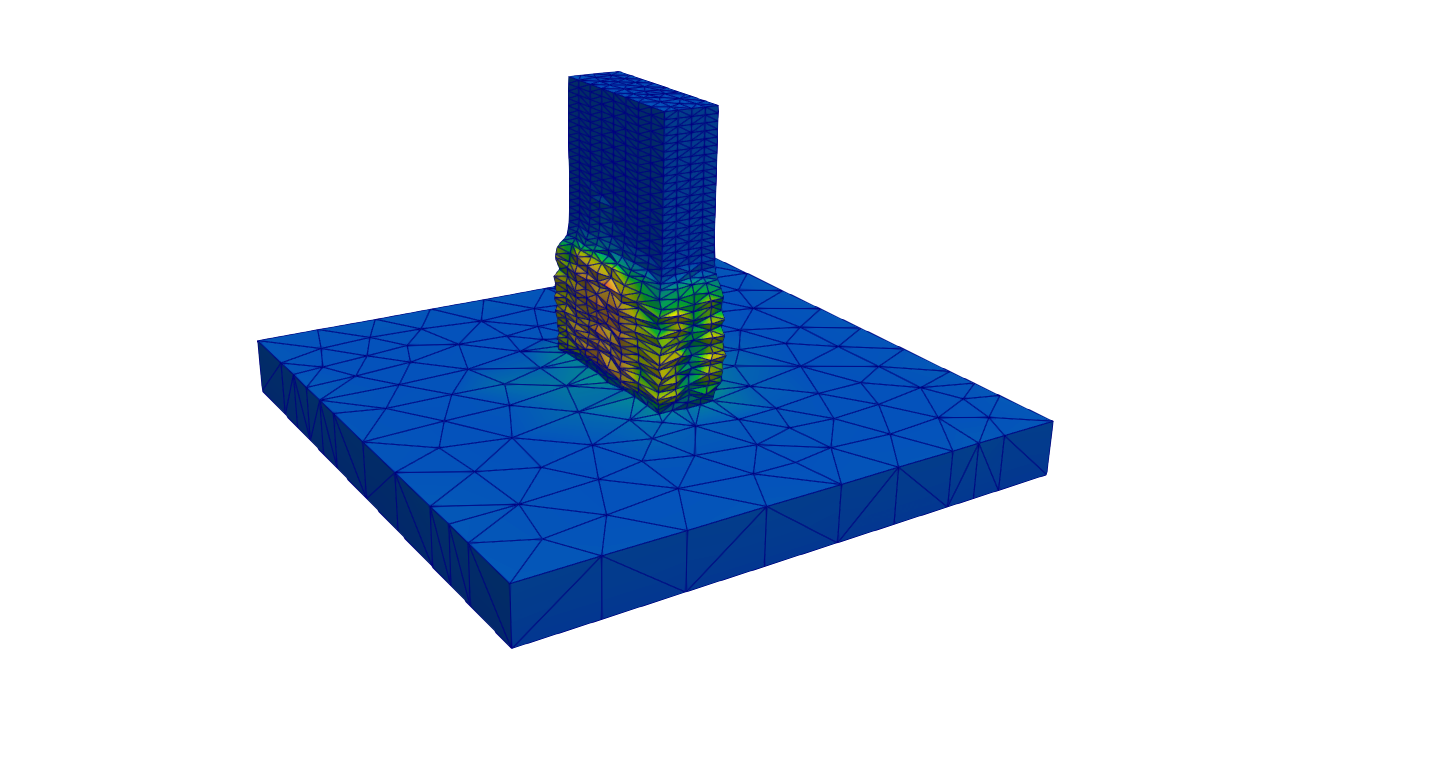
\includegraphics[height=3cm]{fig/4/4.1.6/4.1.6.13.png}
  \caption{时间为0.6,温度场}
  \label{fig:4.1.4:4}
\end{figure}

\begin{figure}[!htbp]
  \centering
  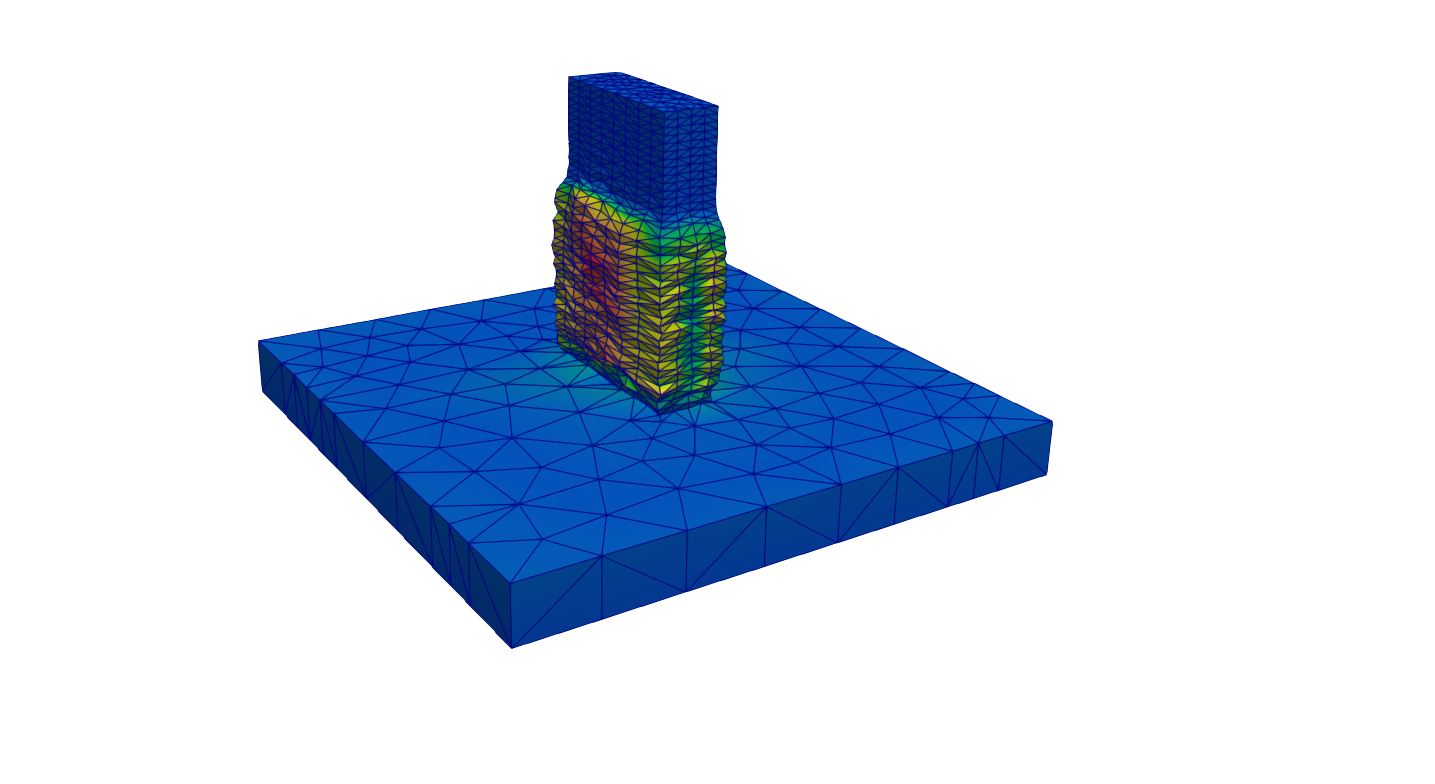
\includegraphics[height=3cm]{fig/4/4.1.6/4.1.6.14.png}
  \caption{时间为0.9,温度场}
  \label{fig:4.1.4:4}
\end{figure}

\begin{figure}[!htbp]
  \centering
  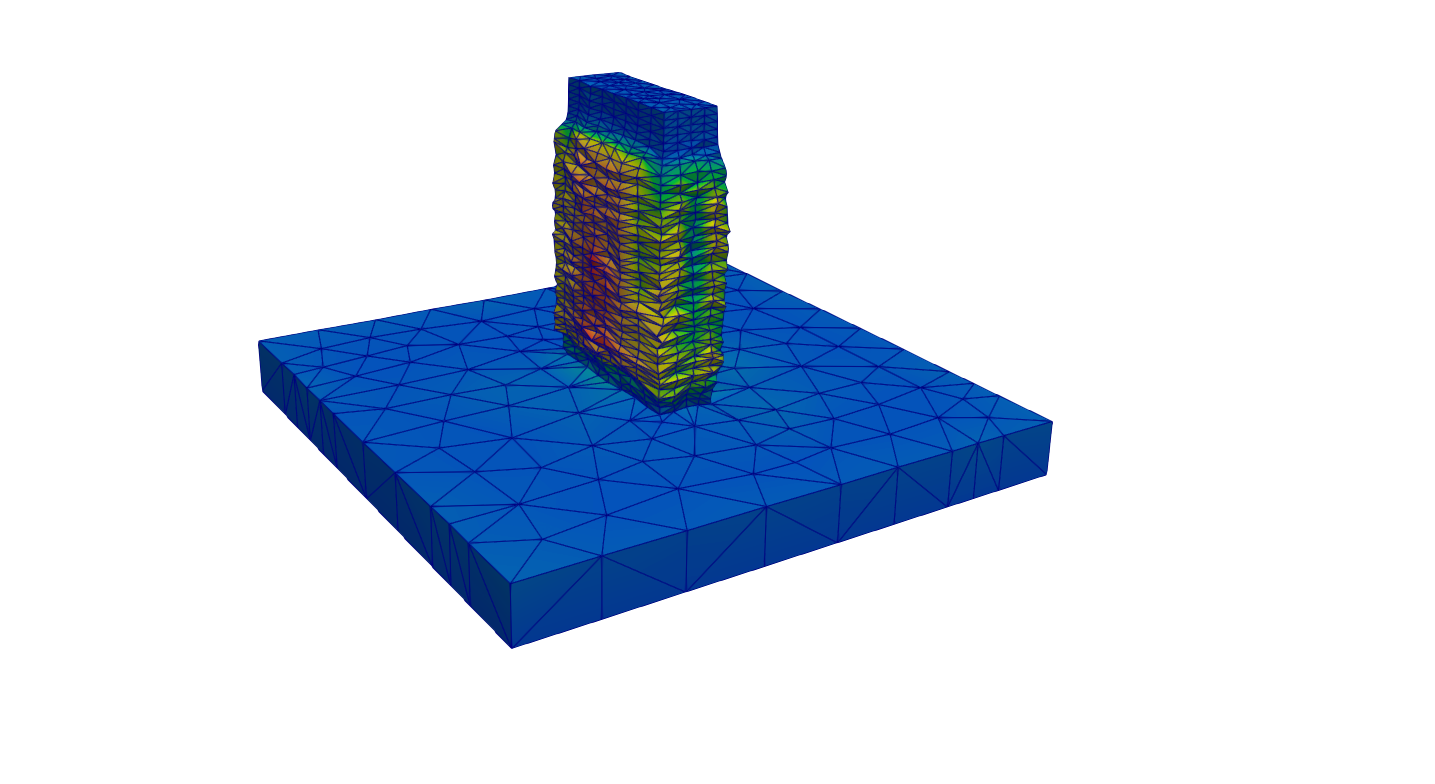
\includegraphics[height=3cm]{fig/4/4.1.6/4.1.6.15.png}
  \caption{时间为1.2,温度场}
  \label{fig:4.1.4:4}
\end{figure}

\begin{figure}[!htbp]
  \centering
  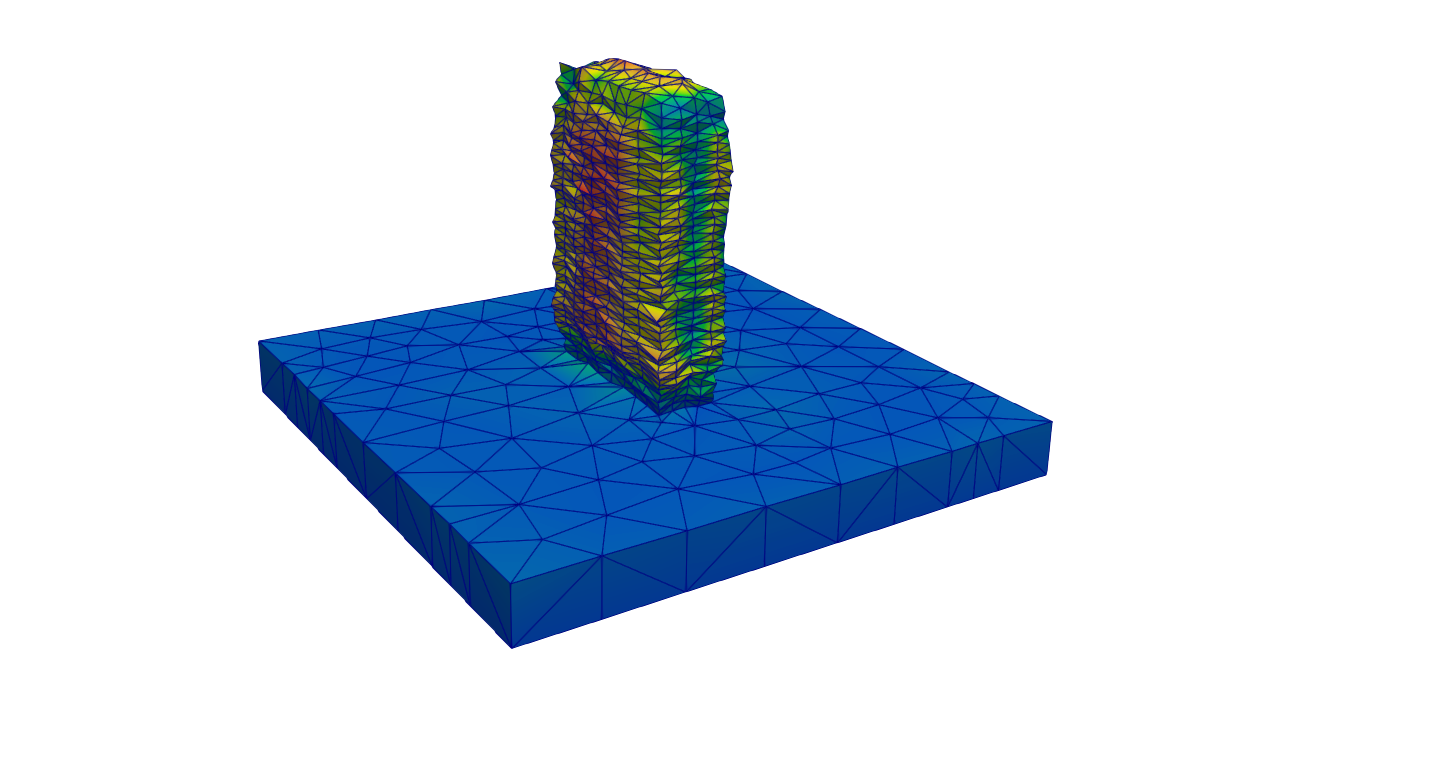
\includegraphics[height=3cm]{fig/4/4.1.6/4.1.6.16.png}
  \caption{时间为1.5,温度场}
  \label{fig:4.1.4:4}
\end{figure}

\begin{figure}[!htbp]
  \centering
  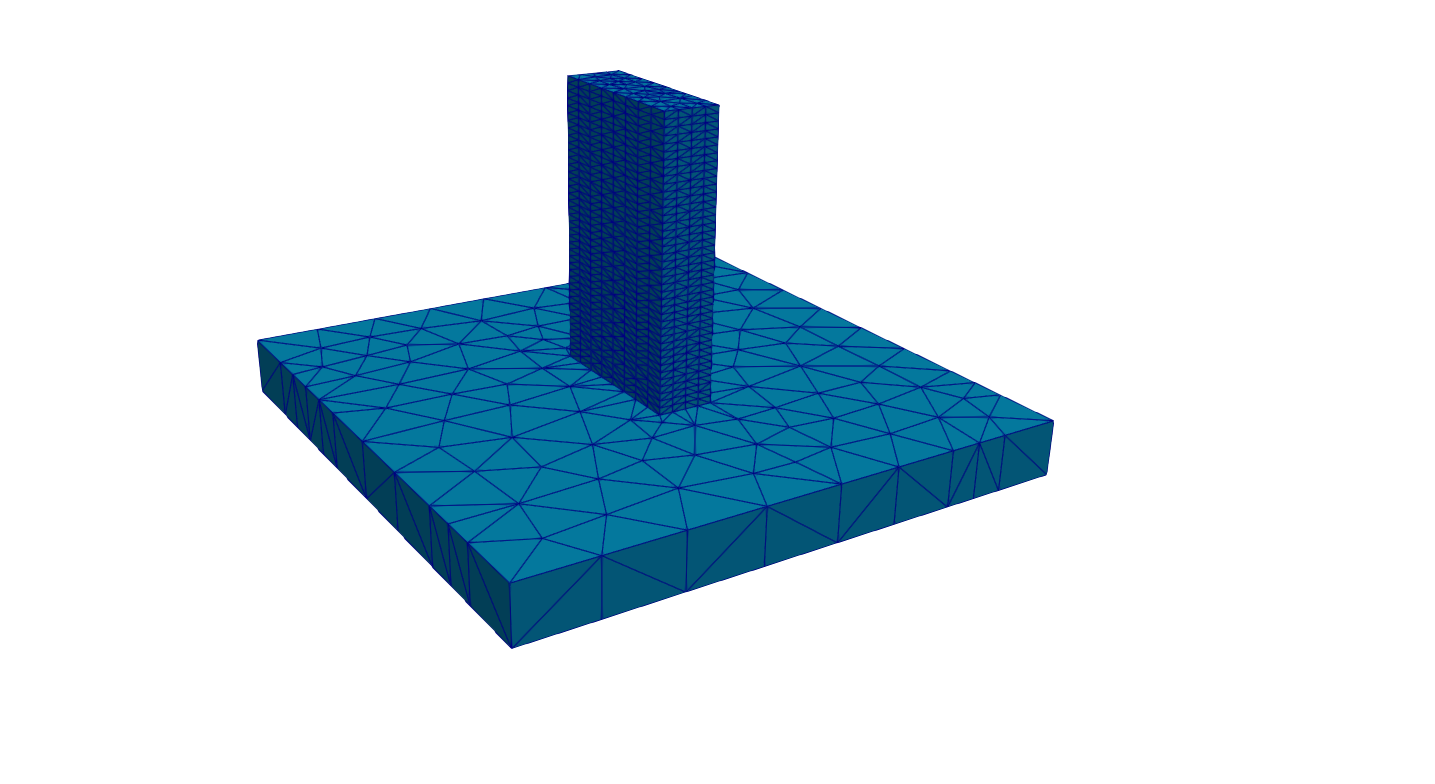
\includegraphics[height=3cm]{fig/4/4.1.6/4.1.6.5.png}
  \caption{时间为0,弹塑性}
  \label{fig:4.1.4:4}
\end{figure}

\begin{figure}[!htbp]
  \centering
  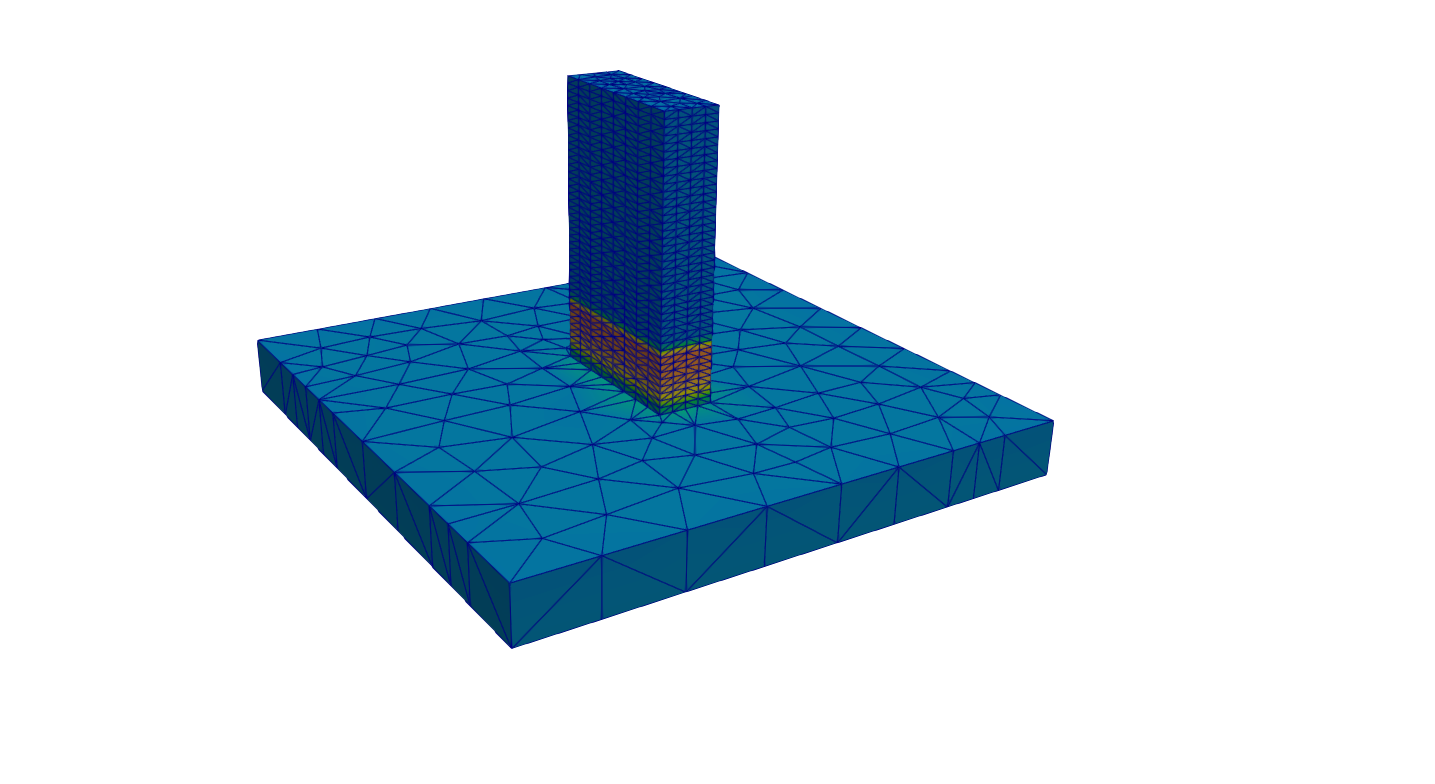
\includegraphics[height=3cm]{fig/4/4.1.6/4.1.6.6.png}
  \caption{时间为0.3,弹塑性}
  \label{fig:4.1.4:4}
\end{figure}

\begin{figure}[!htbp]
  \centering
  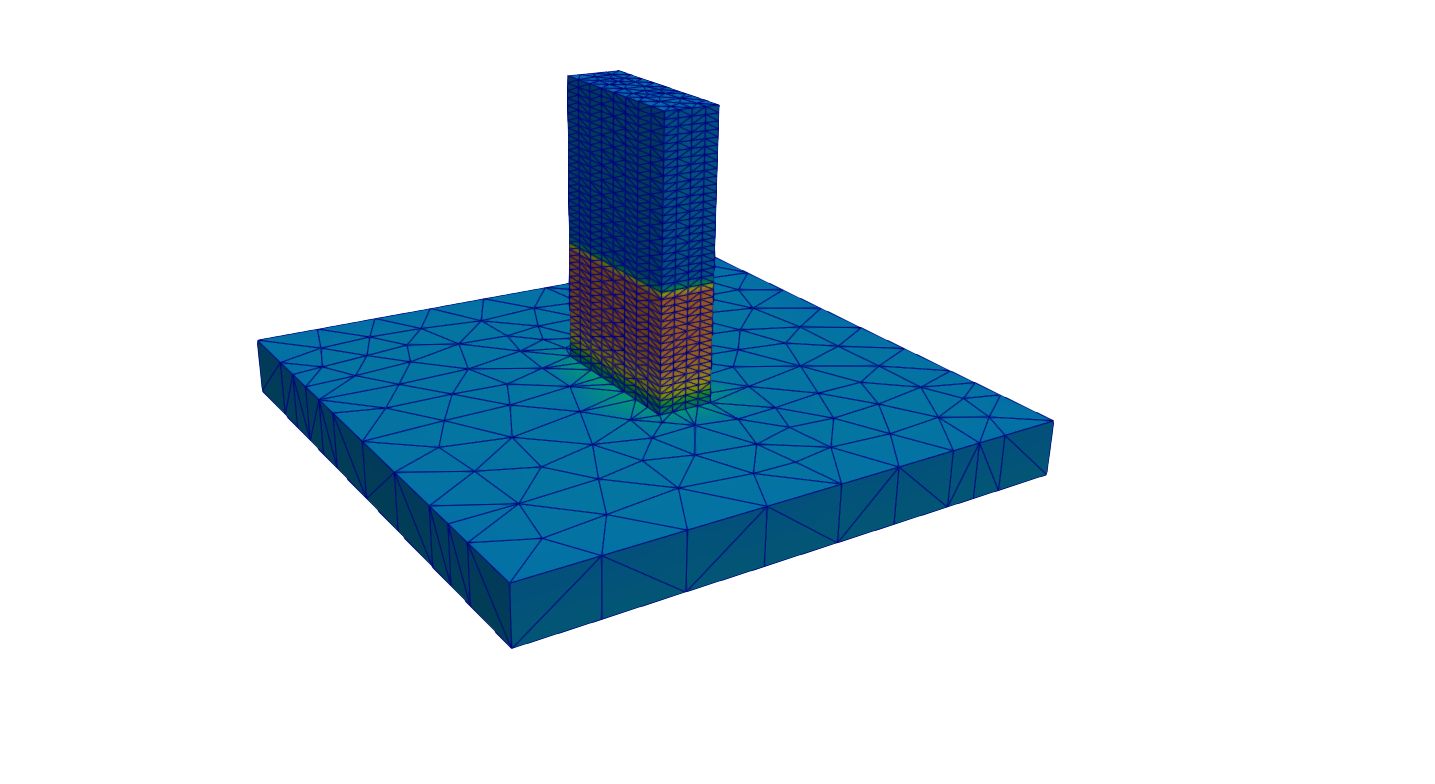
\includegraphics[height=3cm]{fig/4/4.1.6/4.1.6.7.png}
  \caption{时间为0.6,弹塑性}
  \label{fig:4.1.4:4}
\end{figure}

\begin{figure}[!htbp]
  \centering
  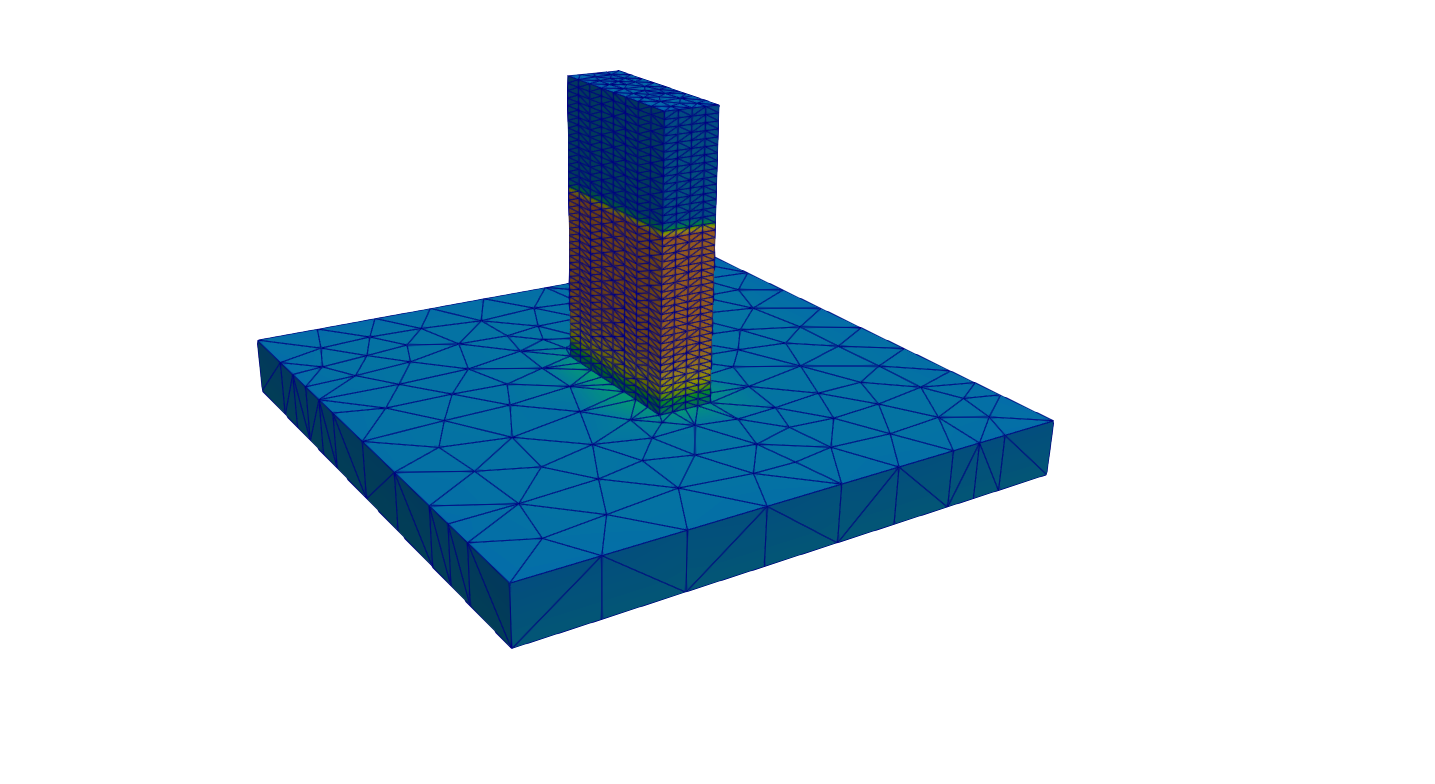
\includegraphics[height=3cm]{fig/4/4.1.6/4.1.6.8.png}
  \caption{时间为0.9,弹塑性}
  \label{fig:4.1.4:4}
\end{figure}

\begin{figure}[!htbp]
  \centering
  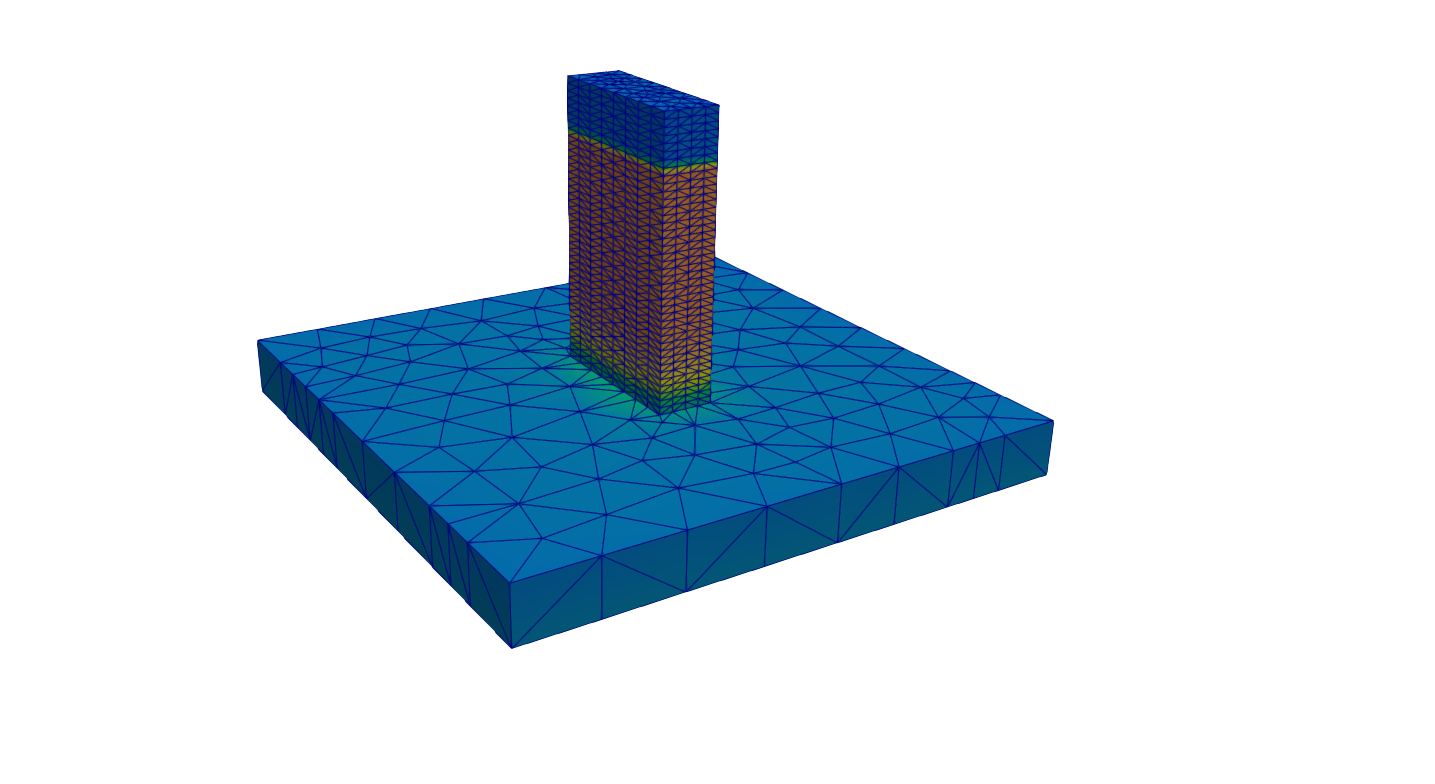
\includegraphics[height=3cm]{fig/4/4.1.6/4.1.6.9.png}
  \caption{时间为1.2,弹塑性}
  \label{fig:4.1.4:4}
\end{figure}

\begin{figure}[!htbp]
  \centering
  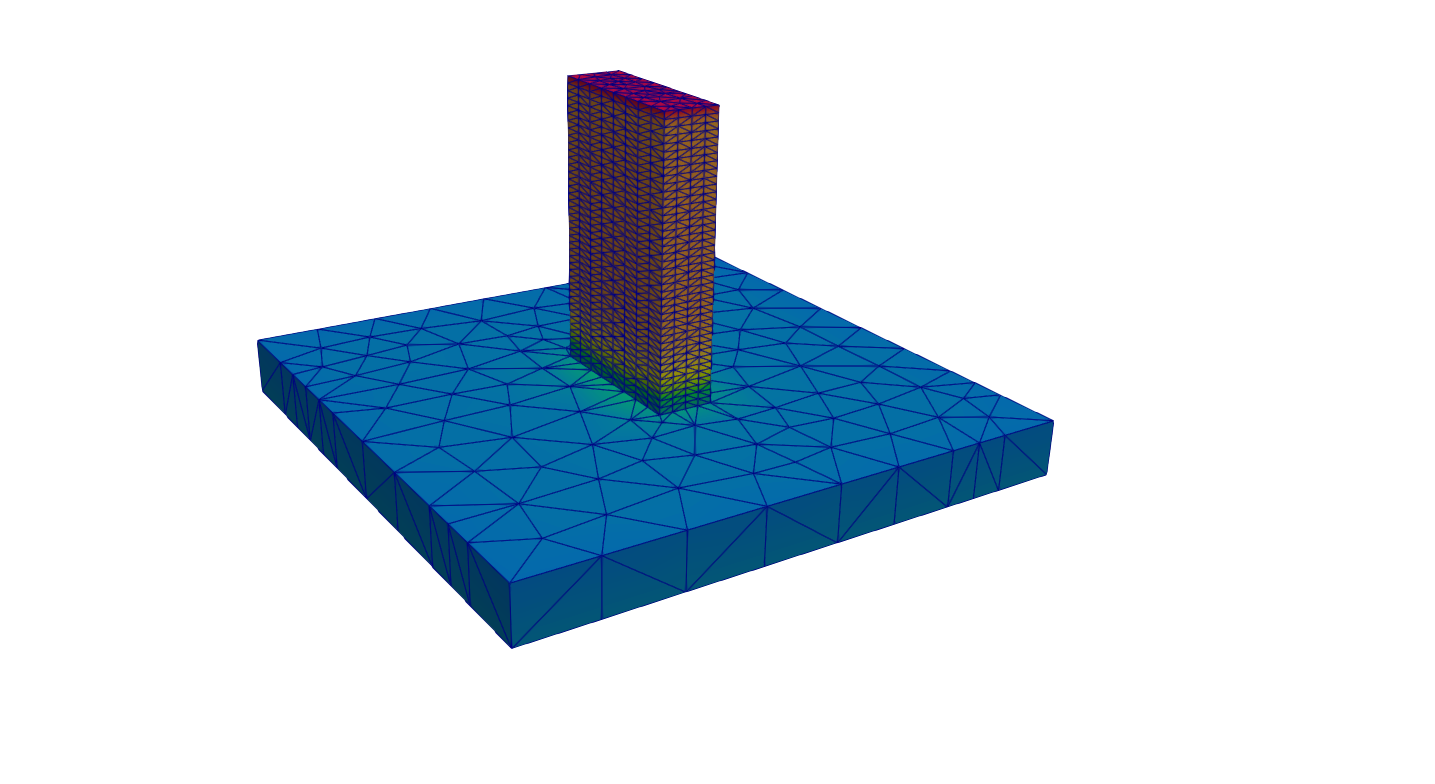
\includegraphics[height=3cm]{fig/4/4.1.6/4.1.6.10.png}
  \caption{时间为1.5,弹塑性}
  \label{fig:4.1.4:4}
\end{figure}



\newpage
\section{构件尺度固有应变法}

\subsection{静态线弹}

线弹性问题的偏微分方程如\eqref{eq:4.1.3:1}。

\begin{align}\label{eq:4.1.3:1}
  -\nabla\cdot\sigma=& \mathbf f  \qquad \mathbf x\in\Omega
\end{align}

Dirichlet边界条件和Neumann边界条件如\eqref{eq:4.1.3:2}。

\begin{subequations}\label{eq:4.1.3:2}
  \begin{align}
    \sigma\cdot\mathbf n =& \mathbf g_{\mathrm N} \qquad \mathbf x\in\Gamma_{\mathrm N}\\
    \mathbf u =& \mathbf g_{\mathrm D} \qquad \mathbf x\in\Gamma_{\mathrm D}
  \end{align}
\end{subequations}

\eqref{eq:4.1.3:1}两边点乘$\mathbf v$,再在$\Omega$上积分得到\eqref{eq:4.1.3:3},通过散度定理得到变分形式\eqref{eq:4.1.3:4}。

\begin{align}\label{eq:4.1.3:3}
  -\int_{\Omega}\nabla\cdot\sigma\cdot\mathbf v\ud x =& \int_{\Omega}\mathbf f\cdot\mathbf v\ud x
\end{align}
  
\begin{align}\label{eq:4.1.3:4}
   \int_{\Omega}\sigma:\varepsilon(\mathbf v)\ud x = \int_{\Omega}\mathbf f\cdot\mathbf v\ud x + \int_{\Gamma}\sigma\cdot\mathbf n\cdot\mathbf v\ud s_x
\end{align}

本构关系如\eqref{eq:4.1.3:5}。

\begin{align}\label{eq:4.1.3:5}
  \sigma(\mathbf u) = 2\mu\mathbf \varepsilon(\mathbf u) + \lambda\mathrm{tr}(\mathbf\varepsilon(\mathbf u))\mathbf I
\end{align}

将\eqref{eq:4.1.3:5}代入\eqref{eq:4.1.3:4}得到\eqref{eq:4.1.3:6}。  
   
\begin{align}\label{eq:4.1.3:6}
  \int_{\Omega}\left(2\mu\mathbf \varepsilon(\mathbf u) :\mathbf\varepsilon(\mathbf v)+\lambda\nabla\cdot\mathbf u \nabla\cdot\mathbf v\right)\ud x =
  \int_{\Gamma}\sigma\cdot\mathbf n\cdot\mathbf v\ud s_x + \int_{\Omega}\mathbf f\cdot\mathbf v\ud x
\end{align}

采用线性单元对\eqref{eq:4.1.3:6}进行离散得到线性方程组\eqref{eq:4.1.3:7}。
   
\begin{align}\label{eq:4.1.3:7}
  KU = b
\end{align}

\eqref{eq:4.1.3:8}定义解析解验证收敛性。

\begin{equation}\label{eq:4.1.3:8}
  \begin{split}
    &\Omega:=(0,1)^3\\
    &\Gamma_{\mathrm D}:=\{x_1=0\}\cup\{x_2=0\}\cup\{x_3=0\} \\
    &\mathbf u = \left(\begin{array}{c} 
      \mathrm e^{x_1+x_2+x_3}\\
      \mathrm e^{x_1+x_2+x_3}\\
      \mathrm e^{x_1+x_2+x_3}
    \end{array}\right)\\
    &\mathbf b = \left(\begin{array}{c}
      -3  (2  \mu + \lambda)  \mathrm e^{x_1+x_2+x_3}\\
      -3  (2  \mu + \lambda)  \mathrm e^{x_1+x_2+x_3}\\
      -3  (2  \mu + \lambda)  \mathrm e^{x_1+x_2+x_3}
    \end{array}\right)\\
    &\mathbf \sigma 
    =\left(\begin{array}{ccc}
      (2\mu + 3\lambda)\mathrm e^{x_1+x_2+x_3} & 2\mu\mathrm e^{x_1+x_2+x_3} & 2\mu\mathrm e^{x_1+x_2+x_3}\\
      2\mu\mathrm e^{x_1+x_2+x_3} & (2\mu + 3\lambda)\mathrm e^{x_1+x_2+x_3} &  2\mu\mathrm e^{x_1+x_2+x_3}\\
      2\mu\mathrm e^{x_1+x_2+x_3} & 2\mu\mathrm e^{x_1+x_2+x_3} & (2\mu + 3\lambda)\mathrm e^{x_1+x_2+x_3}  
    \end{array}\right)
  \end{split}
\end{equation}

图\ref{fig:4.1.3:1}为网格加密3次的结果,表\ref{tab:4.1.3:1}中验证了二次收敛速度。

\begin{figure}[!htbp]
  \centering
  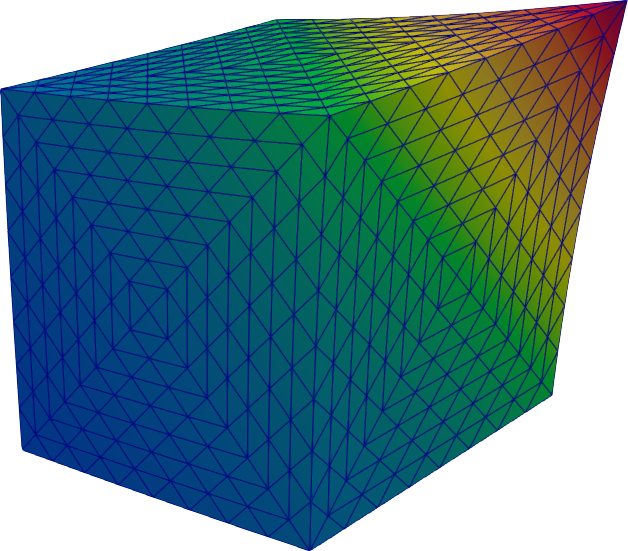
\includegraphics[height=3cm]{fig/4/4.1.3:1.png}
  \caption{三维线弹性方程,弹性模量2.5,泊松比0.25,加密3次,体单元积分点个数为4,边界面单元积分点个数为1}
  \label{fig:4.1.3:1}
\end{figure}

\begin{table}[!htbp]
  \centering
  \begin{tabular}{c|l|l}
    & $\|\mathbf u-\mathbf u_h\|_{L^2}$ & ROC\\
    \hline
    3 & 0.0002305107    & \\
    \hline
    4 & 0.0000581654   & 3.963020971  \\
    \hline
    5 & 0.0000145494  &  3.99778685 \\
    \hline
    6 & 0.0000036350 &  4.00258597
  \end{tabular}
  \label{tab:4.1.3:1}
  \caption{三维线弹性方程,弹性模量2.5,泊松比0.25,体单元积分点个数为4,边界面单元积分点个数为1。}
\end{table}

图\ref{fig:4.1.3:1}为网格加密3次的结果,表\ref{tab:4.1.3:1}中验证了二次收敛速度。

\begin{figure}[!htbp]
  \centering
  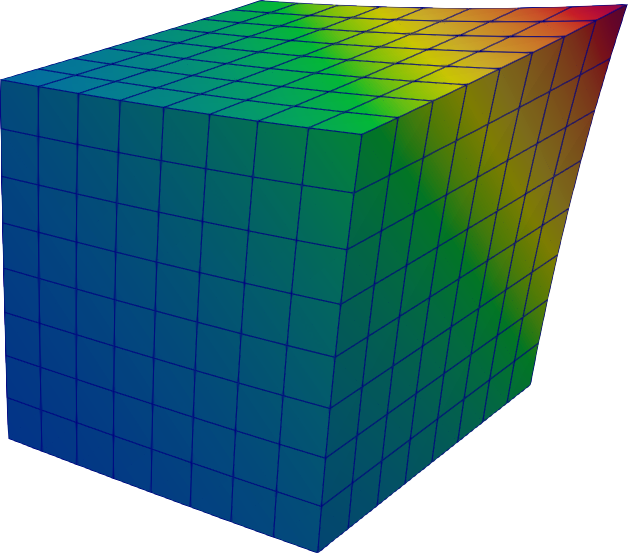
\includegraphics[height=3cm]{fig/4/4.1.3:2.png}
  \caption{三维线弹性方程,弹性模量2.5,泊松比0.25,加密3次,体单元积分点个数为1,边界面单元积分点个数为1}
  \label{fig:4.1.3:2}
\end{figure}

\begin{table}[!htbp]
  \centering
  \begin{tabular}{c|l|l}
    & $\|\mathbf u-\mathbf u_h\|_{L^2}$ & ROC\\
    \hline
    3 &  0.0004850991   & \\
    \hline
    4 & 0.0001214924   &  3.992834943 \\
    \hline
    5 & 0.0000303867  &   3.998209743 \\
    \hline
    6 & 0.0000075975 &  3.999565647
  \end{tabular}
  \label{tab:4.1.3:1}
  \caption{三维线弹性方程,弹性模量2.5,泊松比0.25,体单元积分点个数为1,边界面单元积分点个数为1。}
\end{table}


\subsection{动态线弹}

瞬态线弹性问题的偏微分方程如\eqref{eq:4.1.4:1}。

\begin{align}\label{eq:4.1.4:1}
  \rho\ddot{\mathbf u}-\nabla\cdot\sigma=& \mathbf f \qquad \mathbf x\in\Omega
\end{align}

初始条件如\eqref{eq:4.1.4:2}。 
	
\begin{equation}\label{eq:4.1.4:2}
  \begin{split}
    \mathbf u(0,\mathbf x) = & \mathbf h_1 \qquad \mathbf x\in\overline\Omega\\
    \dot{\mathbf u}(0,\mathbf x) = & \mathbf h_2 \qquad \mathbf x\in\overline\Omega
  \end{split}
\end{equation}

采用线性单元进行离散得到线性方程组\eqref{eq:4.1.4:3}。

\begin{align}\label{eq:4.1.4:3}
   M U'' + KU = b
\end{align}

\begin{align*}
  M\frac{\frac{U^{n+1}-U^{n}}{h}-\frac{U^{n}-U^{n-1}}{h}}{h} + KU^{n+1} =& b^{n+1}\\
  MU^{n+1} + h^2KU^{n+1} =& 2MU^{n} - MU^{n-1} + h^2b^{n+1}
\end{align*}

通过解析解\eqref{eq:4.1.4:4}验证收敛性。

\begin{equation}\label{eq:4.1.4:4}
  \begin{split}
    &\Omega:=(0,1)^3\\
    &\Gamma_{\mathrm D}:=\{x_1=0\}\cup\{x_2=0\}\cup\{x_3=0\} \\
    &\mathbf u = \mathrm e^t \left(\begin{array}{c} 
      \mathrm e^{x_1+x_2+x_3}\\
      \mathrm e^{x_1+x_2+x_3}\\
      \mathrm e^{x_1+x_2+x_3}
    \end{array}\right)\\
    &\mathbf b = \mathrm e^t\left(\begin{array}{c}
      (1-3  (2  \mu + \lambda))  \mathrm e^{x_1+x_2+x_3}\\
      (1-3  (2  \mu + \lambda))  \mathrm e^{x_1+x_2+x_3}\\
      (1-3  (2  \mu + \lambda))  \mathrm e^{x_1+x_2+x_3}
    \end{array}\right)\\
    &\mathbf \sigma 
    =\mathrm e^t\left(\begin{array}{ccc}
      (2\mu + 3\lambda)\mathrm e^{x_1+x_2+x_3} & 2\mu\mathrm e^{x_1+x_2+x_3} & 2\mu\mathrm e^{x_1+x_2+x_3}\\
      2\mu\mathrm e^{x_1+x_2+x_3} & (2\mu + 3\lambda)\mathrm e^{x_1+x_2+x_3} &  2\mu\mathrm e^{x_1+x_2+x_3}\\
      2\mu\mathrm e^{x_1+x_2+x_3} & 2\mu\mathrm e^{x_1+x_2+x_3} & (2\mu + 3\lambda)\mathrm e^{x_1+x_2+x_3}  
    \end{array}\right)
  \end{split}
\end{equation}


图\ref{fig:4.1.4:1}和\ref{fig:4.1.4:2}为网格加密3次和时间加密5次的结果,表中验证了二次收敛速度。

\begin{figure}[!htbp]
  \centering
  \includegraphics[height=3cm]{fig/4/4.1.4/1.png}
  \caption{三维线弹性方程,动态隐式,弹性模量2.5,泊松比0.25,网格加密3次,时间加密5次,体单元积分点个数为1,边界单元积分点个数为1,时间0。}
  \label{fig:4.1.4:1}
\end{figure}

\begin{figure}[!htbp]
  \centering
  \includegraphics[height=3cm]{fig/4/4.1.4/2.png}
  \caption{三维线弹性方程,动态隐式,弹性模量2.5,泊松比0.25,网格加密3次,时间加密5次,体单元积分点个数为1,边界单元积分点个数为1,时间0.5。}
  \label{fig:4.1.4:2}
\end{figure}


\begin{table}[!htbp]
  \centering
  \begin{tabular}{c|l|l}
    & $\|\mathbf u-\mathbf u_h\|_{L^2}$ & ROC\\
    \hline
    2,3 & 0.00279 &  \\
    \hline
    3,5 & 0.00094    & 2.968085106 \\
    \hline
    4,7 & 0.00025   &     3.76
  \end{tabular}
  \caption{三维线弹性方程,动态隐式,弹性模量2.5,泊松比0.25,体单元积分点个数为1,边界单元积分点个数为1,时间0.5。}
\end{table}

图\ref{fig:4.1.4:3}和\ref{fig:4.1.4:4}为网格加密3次和时间加密5次的结果,表中验证了二次收敛速度。

\begin{figure}[!htbp]
  \centering
  \includegraphics[height=3cm]{fig/4/4.1.4/3.png}
  \caption{三维线弹性方程,动态隐式,弹性模量2.5,泊松比0.25,网格加密3次,时间加密5次,体单元积分点个数为1,边界单元积分点个数为1,时间0。}
  \label{fig:4.1.4:3}
\end{figure}

\begin{figure}[!htbp]
  \centering
  \includegraphics[height=3cm]{fig/4/4.1.4/4.png}
  \caption{三维线弹性方程,动态隐式,弹性模量2.5,泊松比0.25,网格加密3次,时间加密5次,体单元积分点个数为1,边界单元积分点个数为1,时间0.5。}
  \label{fig:4.1.4:4}
\end{figure}


\begin{table}[!htbp]
  \centering
  \begin{tabular}{c|l|l}
    & $\|\mathbf u-\mathbf u_h\|_{L^2}$ & ROC\\
    \hline
    2,3 & 0.00463 &  \\
    \hline
    3,5 & 0.00158    &  2.930379747\\
    \hline
    4,7 & 0.00042   &     3.761904762
  \end{tabular}
  \caption{三维线弹性方程,动态隐式,弹性模量2.5,泊松比0.25,体单元积分点个数为1,边界单元积分点个数为1,时间0.5。}
\end{table}

\begin{figure}[!htbp]
  \centering
  \includegraphics[height=6cm]{fig/4/4.1.6/engine1.png}
  \caption{网格单元为5370240}
  \label{fig:4.1.3:1}
\end{figure}

\begin{figure}[!htbp]
  \centering
  \includegraphics[height=6cm]{fig/4/4.1.6/engine2.png}
  \caption{网格单元为5370240}
  \label{fig:4.1.3:1}
\end{figure}

\begin{figure}[!htbp]
  \centering
  \includegraphics[height=6cm]{fig/4/4.1.6/engine3.png}
  \caption{火箭推进室打印}
  \label{fig:4.1.3:1}
\end{figure}
